% Versão 24/06/2020

% Este documento destina-se a servir como modelo para a produção de documentos
% de pesquisa do PPGINF/UFPR, como projetos, dissertações e teses. A classe de
% documento se chama "ppginf" (arquivo ppginf.cls) e define o formato básico do
% documento. O texto está organizado em capítulos que são colocados em
% subdiretórios separados. São definidos exemplos para a inclusão de figuras,
% códigos-fonte e a definição de tabelas.
%
% Produzido por Carlos Maziero (maziero@inf.ufpr.br).

%=====================================================

% Opções da classe ppginf:
%
% - defesa    : versão para entregar à banca; tem espaçamento 1,5
%               e omite algumas páginas iniciais (agradecimentos, etc)
% - final     : versão pós-defesa, para enviar à biblioteca;
%               tem espaçamento simples e todas as páginas iniciais.
% - oneside   : somente frente; use quando for gerar somente o PDF.
% - twoside   : frente/verso; use se precisar de uma versão impressa.
% - metadados : inclui metadados no PDF (por default não inclui)
% - ...       : demais opções aceitas pela classe "book"

% ATENÇÂO: este modelo tem suporte para português e inglês.
% As duas línguas devem ser informadas como opção da classe;
% a língua principal do documento deve vir POR ÚLTIMO.

% Versão de defesa
\documentclass[defesa,oneside,english,brazilian]{ppginf}

% Versão de defesa em inglês
%\documentclass[defesa,oneside,brazilian,english]{ppginf}

% Versão final em PDF para a biblioteca da UFPR
%\documentclass[final,oneside,english,brazilian]{ppginf}

% Versão final para impressão (frente/verso)
%\documentclass[final,twoside,english,brazilian]{ppginf}

% configurações de diversos pacotes, inclusive a fonte usada no texto
% Pacotes usados neste documento e suas respectivas configurações

% ------------------------------------------------------------------------------

% Definição de fontes

% formato dos arquivos-fonte (utf8 no Linux e latin1 no Windows)
\usepackage[utf8]{inputenc}	% arquivos LaTeX em Unicode (UTF8)

% usar codificação T1 para ter caracteres acentuados corretos no PDF
\usepackage[T1]{fontenc}

% fonte usada no corpo do texto (pode alterar, mas descomente apenas uma)
\usepackage{newtxtext,newtxmath}	% Times (se não tiver, use mathptmx)
%\usepackage{lmodern}			% Computer Modern (fonte clássico LaTeX)
%\usepackage{kpfonts}			% Kepler/Palatino (idem, use mathpazo)
%\renewcommand{\familydefault}{\sfdefault} % Arial/Helvética (leia abaixo)

% A biblioteca central da UFPR recomenda usar Arial, seguindo a recomendação da
% ABNT. Essa é uma escolha ruim, pois fontes sans-serif são geralmente inade-
% quados para textos longos e impressos, sendo melhores para páginas Web.
% http://www.webdesignerdepot.com/2013/03/serif-vs-sans-the-final-battle/.

% fontes usadas em ambientes específicos
\usepackage[scaled=0.9]{helvet}		% Sans Serif
\usepackage{courier}			% Verbatim, Listings, etc

% ------------------------------------------------------------------------------

% inclusão de figuras em PDF, PNG, PS, EPS
\usepackage{graphicx}

% subfiguras (subfigure is deprecated, don't use it)
\usepackage[labelformat=simple]{subcaption}
\renewcommand\thesubfigure{(\alph{subfigure})}

% ------------------------------------------------------------------------------

% inclusão/formatação de código-fonte (programas)
\usepackage{listings}
\lstset{language=c}
\lstset{basicstyle=\ttfamily\footnotesize,commentstyle=\textit,stringstyle=\ttfamily}
\lstset{showspaces=false,showtabs=false,showstringspaces=false}
\lstset{numbers=left,stepnumber=1,numberstyle=\tiny}
\lstset{columns=flexible,mathescape=true}
\lstset{frame=single}
\lstset{inputencoding=utf8,extendedchars=true}
\lstset{literate={á}{{\'a}}1  {ã}{{\~a}}1 {à}{{\`a}}1 {â}{{\^a}}1
                 {Á}{{\'A}}1  {Ã}{{\~A}}1 {À}{{\`A}}1 {Â}{{\^A}}1
                 {é}{{\'e}}1  {ê}{{\^e}}1 {É}{{\'E}}1  {Ê}{{\^E}}1
                 {í}{{\'\i}}1 {Í}{{\'I}}1
                 {ó}{{\'o}}1  {õ}{{\~o}}1 {ô}{{\^o}}1
                 {Ó}{{\'O}}1  {Õ}{{\~O}}1 {Ô}{{\^O}}1
                 {ú}{{\'u}}1  {Ú}{{\'U}}1
                 {ç}{{\c{c}}}1 {Ç}{{\c{C}}}1 }

% ------------------------------------------------------------------------------

% formatação de algoritmos
\usepackage{algorithm,algorithmic}
\IfLanguageName{brazilian} {\floatname{algorithm}{Algoritmo}}{}
\renewcommand{\algorithmiccomment}[1]{~~~// #1}
%\algsetup{linenosize=\footnotesize,linenodelimiter=.}

% ------------------------------------------------------------------------------

% formatação de bibliografia
\usepackage{natbib}		% bibliografia no estilo NatBib
\renewcommand{\cite}{\citep}	% \cite deve funcionar como \citep
%\bibpunct{[}{]}{;}{a}{}{,}	% caracteres usados nas referências

% ------------------------------------------------------------------------------

% fontes adicionais
\usepackage{amsmath}		% pacotes matemáticos
\usepackage{amsfonts}		% fontes matemáticas 
\usepackage{amssymb}		% símbolos 

% ------------------------------------------------------------------------------

% pacotes diversos
\usepackage{alltt,moreverb}	% mais comandos no modo verbatim
\usepackage{lipsum}		% gera texto aleatório (para os exemplos)
\usepackage{currfile}		% infos sobre o arquivo/diretório atual
\usepackage[final]{pdfpages}	% inclusão de páginas em PDF
\usepackage{longtable}		% tabelas multi-páginas (tab símbolos/acrônimos)

% ------------------------------------------------------------------------------



%=====================================================

\begin {document}

% Principais dados, usados para gerar as páginas iniciais.
% Campos não utilizados podem ser removidos ou comentados.

% título
\title{Testes de hipótese em Modelos Multivariados \\ de Covariância Linear Generalizada (McGLM)}

% palavras-chave e keywords (p/ resumo, abstract e metadados do PDF)
\pchave{Palavra-chave 1. Palavra-chave 2. Palavra-chave 3.}
\keyword{Keyword 1. Keyword 2. Keyword 3.}

% autoria
\author{Lineu Alberto Cavazani de Freitas}
\advisor{Prof. Dr. Wagner Hugo Bonat}
\coadvisor{Prof. Dr. Marco Antonio Zanata Alves}

% instituição
\IfLanguageName{brazilian}
  { \instit{UFPR}{Universidade Federal do Paraná} }
% a Bib/UFPR exige que tudo seja em português, exceto o título :-(
%  { \instit{UFPR}{Federal University of Paraná} }
  { \instit{UFPR}{Universidade Federal do Paraná} }

% área de concentração (default do PPGInf, não mudar)
\IfLanguageName{brazilian}
  { \field{Ciência da Computação} }
% a Bib/UFPR exige que tudo seja em português, exceto o título :-(
%  { \field{Computer Science} }
  { \field{Ciência da Computação} }

% data (só o ano)
\date{2021}

% local
\IfLanguageName{brazilian}
  { \local{Curitiba PR} }
% a Bib/UFPR exige que tudo seja em português, exceto o título :-(
%  { \local{Curitiba PR - Brazil} }
  { \local{Curitiba PR} }

% imagem de fundo da capa (se não desejar, basta comentar)
\coverimage{0-iniciais/fundo-capa.jpg}

%=====================================================

%% Descrição do documento (obviamente, descomentar somente UMA!)

% Por exigência da biblioteca da UFPR, a descrição do documento deve ser
% em português, mesmo em documentos em outras línguas. Vá entender...

% tese de doutorado
\descr{Documento apresentado como requisito parcial ao exame de qualificação de Mestrado no Programa de Pós-Graduação em Informática, Setor de Ciências Exatas, da Universidade Federal do Paraná}

% exame de qualificação de doutorado
%\descr{Documento apresentado como requisito parcial ao exame de qualificação de Doutorado no Programa de Pós-Graduação em Informática, Setor de Ciências Exatas, da Universidade Federal do Paraná}

% dissertação de mestrado
%\descr{Dissertação apresentada como requisito parcial à obtenção do grau de Mestre em Informática no Programa de Pós-Graduação em Informática, Setor de Ciências Exatas, da Universidade Federal do Paraná}

% exame de qualificação de mestrado
%\descr{Documento apresentado como requisito parcial ao exame de qualificação de Mestrado no Programa de Pós-Graduação em Informática, Setor de Ciências Exatas, da Universidade Federal do Paraná}

% trabalho de conclusão de curso
%\descr{Trabalho apresentado como requisito parcial à conclusão do Curso de Bacharelado em XYZ, Setor de Ciências Exatas, da Universidade Federal do Paraná}

% trabalho de disciplina
%\descr{Trabalho apresentado como requisito parcial à conclusão da disciplina XYZ no Curso de Bacharelado em XYZ, Setor de Ciências Exatas, da Universidade Federal do Paraná}

% doctorate thesis
%\descr{Thesis presented as a partial requirement for the degree of Doctor in Computer Science in the Graduate Program in Informatics, Exact Sciences Sector, of the Federal University of Paraná, Brazil}

% doctorate qualification
%\descr{Document presented as a partial requirement for the doctoral qualification exam in the Graduate Program in Informatics, Exact Sciences Sector, of the Federal University of Paraná, Brazil}

% MSc dissertation
%\descr{Dissertation presented as a partial requirement for the degree of Master of Sciences in Informatics in the Graduate Program in Informatics, Exact Sciences Sector, of the Federal University of Paraná, Brazil.}

% MSc qualification
%\descr{Document presented as a partial requirement for the Master of Sciences qualification exam in the Graduate Program in Informatics, Exact Sciences Sector, of the Federal University of Paraná, Brazil}

%=====================================================

% define estilo das páginas iniciais (capas, resumo, sumário, etc)
\frontmatter
\pagestyle{frontmatter}

% produz capa e folha de rosto
\titlepage

% páginas que só aparecem na versão final (a inclusão é automática)
% IMPORTANTE: o conteúdo exato da ficha catalográfica é preparada pela
% Biblioteca da UFPR. Não "invente" um conteúdo para ela!

\begin{ficha}	% só gera conteúdo se for na versão final

% inclusão da ficha catalográfica final (arquivo PDF)
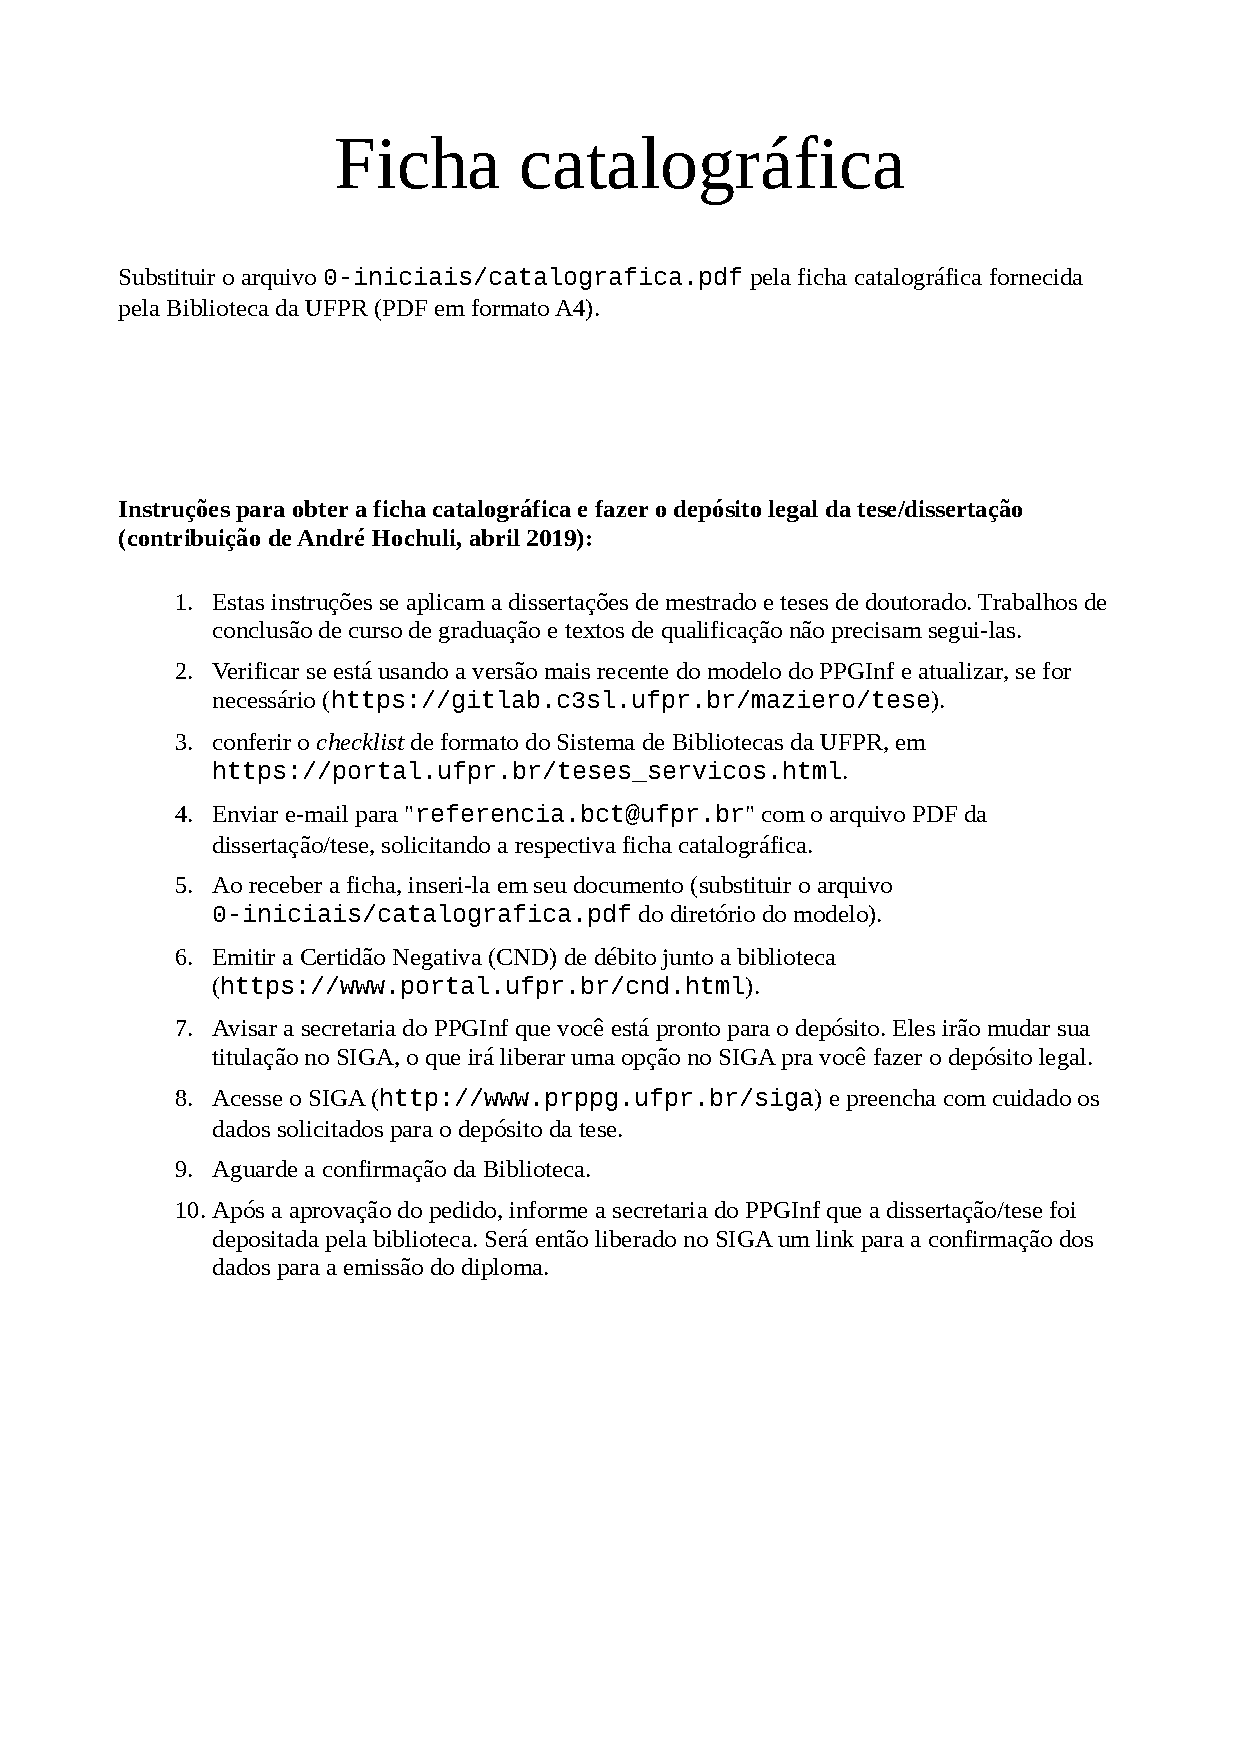
\includepdf[noautoscale]{0-iniciais/catalografica.pdf}

\end{ficha}

%=====================================================
	% ficha catalográfica
% A ficha de aprovação será fornecida pela secretaria do programa,
% após a defesa e cumprimento dos demais trâmites legais.

\begin{aprovacao}	% só gera conteúdo se for na versão final

% inclusão do termo de aprovação final (arquivo PDF)
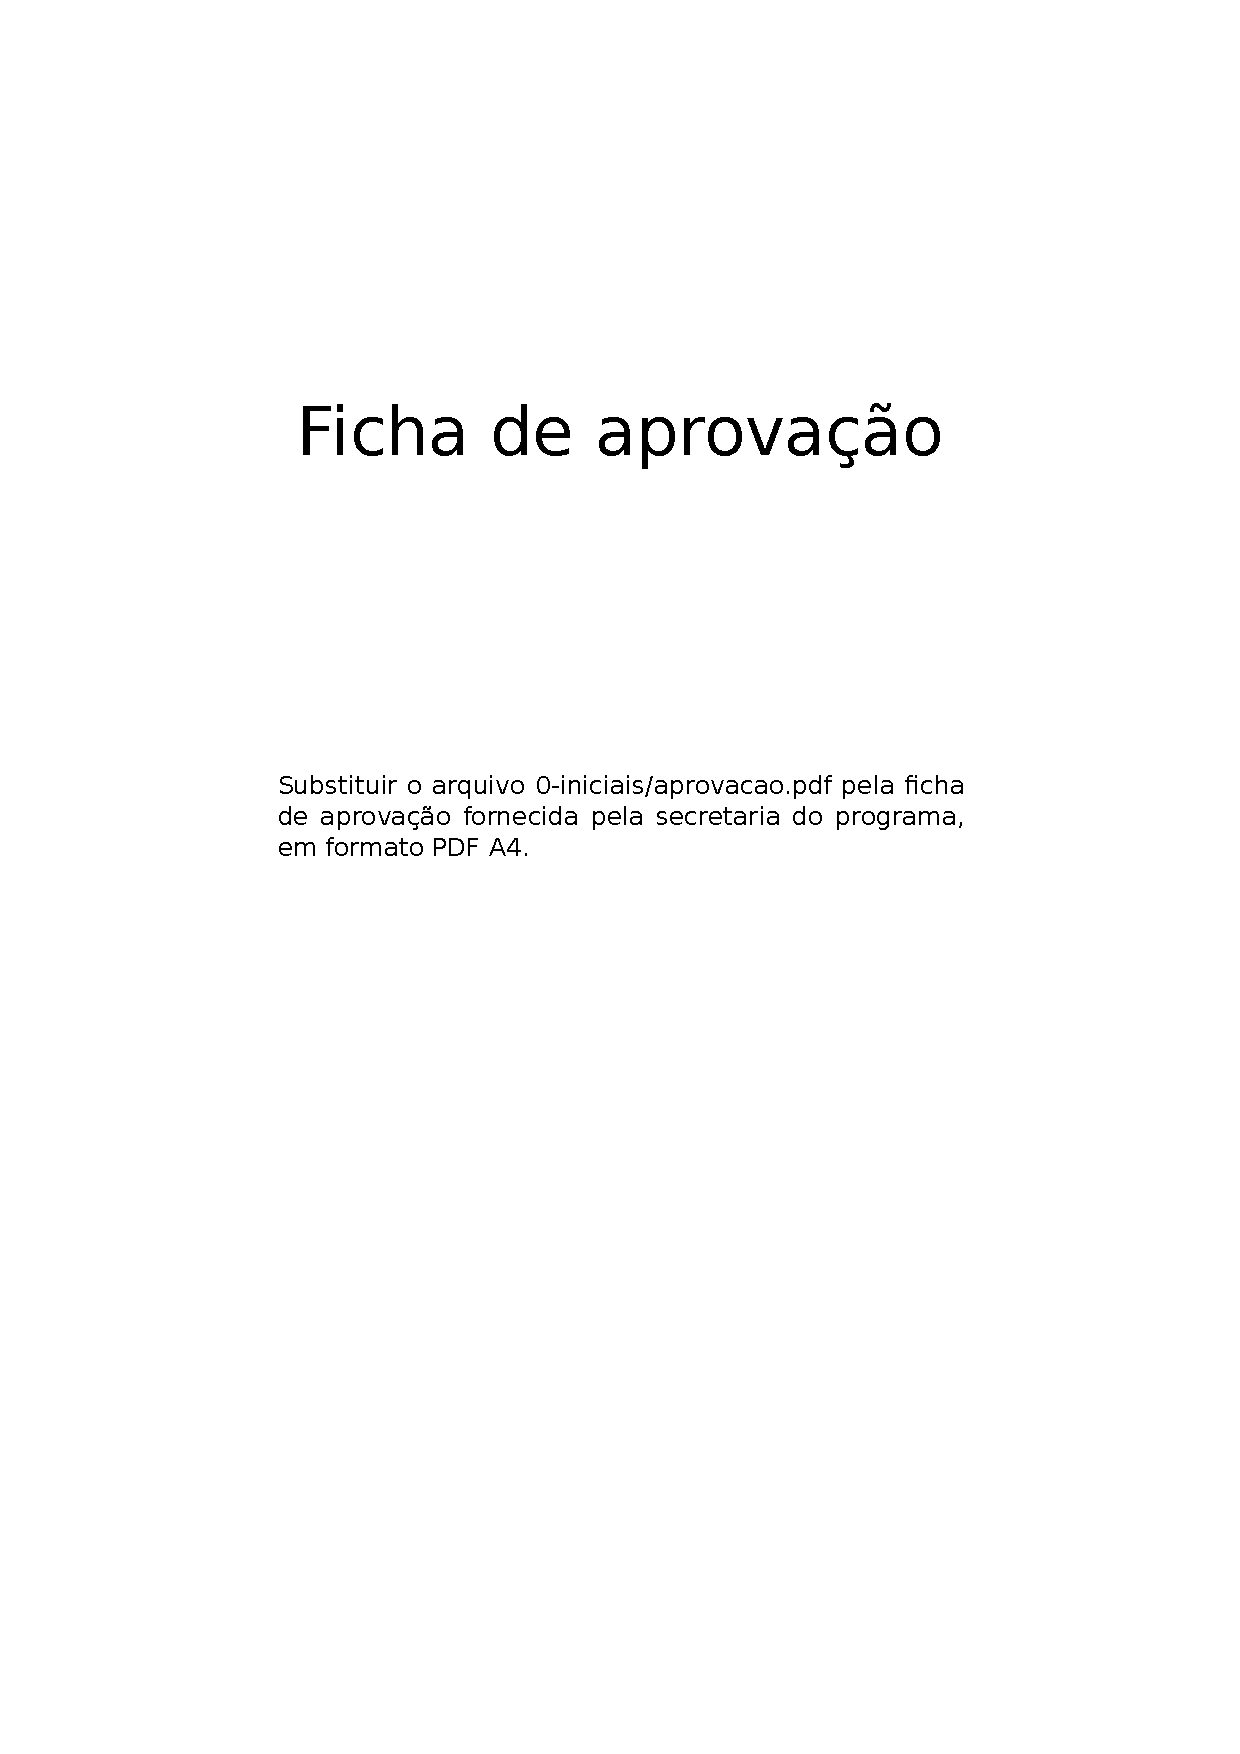
\includepdf[noautoscale]{0-iniciais/aprovacao.pdf}

\end{aprovacao}

%=====================================================
		% folha de aprovação
\begin{dedica}  % só gera conteúdo se for na versão final

A alguém...

\end{dedica}

		% dedicatória
\begin{agradece}	% só gera conteúdo se for na versão final

Inserir os agradecimentos. Os agradecimentos devem ocupar no máximo uma página, devem ser justificados na largura da página e com um afastamento de parágrafo na primeira linha de 1,27 cm. O espaçamento entre linhas deve ser de 1,5 linhas. Não deve haver espaçamento adicional entre parágrafos.

\lipsum[2-5]	% gera um texto aleatório

\end{agradece}

		% agradecimentos

% resumo (português) e abstract (inglês)
\begin{resumo}

Ciência de dados é um campo de estudo interdisciplinar que compreende áreas como estatística, ciência da computação e matemática. Neste contexto, métodos estatísticos são de fundamental importância sendo que, dentre as possíveis técnicas disponíveis para análise de dados, os modelos de regressão tem papel importante. Tais modelos são indicados a problemas nos quais existe interesse em verificar a associação entre uma ou mais variáveis respostas e um conjunto de variáveis explicativas; isto é feito através da obtenção de uma equação que explique a relação entre as variáveis explicativas e a(s) resposta(s). Existem modelos uni e multivariados: nos modelos univariados há apenas uma variável resposta; já em modelos multivariados há mais de uma resposta. Dentre as classes de modelos multivariados estão os modelos multivariados de covariância linear generalizada (McGLMs). Trata-se de uma flexível clase que permite lidar com múltiplas respostas de diferentes naturezas, correlacionadas entre si em que é possível modelar também a correlação entre indivíduos do conjunto de dados. No contexto de modelos de regressão, um interesse comum costuma ser verificar se a retirada de determinada variável explicativa gera um modelo significativamente pior, ou seja, avalia-se se há evidência suficiente nos dados para afirmar que determinada variável explicativa não possui efeito sobre a resposta. Tais conjecturas são avaliadas através dos chamados testes de hipóteses. Três testes de hipóteses são comuns em regressão: o teste da razão de verossimilhanças, o teste Wald e o teste do multiplicador de lagrange, também conhecido como teste escore. Existem ainda técnicas baseadas em testes de hipóteses tais como a análise de variância (ANOVA) em que o objetivo é a avaliação do efeito de cada uma das variáveis explicativas sobre a(s) resposta(s); isto é feito através da comparação via testes de hipóteses entre modelos com e sem cada uma das variáveis explicativas. Para o caso multivariado estende-se a técnica de análise de variância (ANOVA) para a análise de variância  multivariada (MANOVA). No entanto, considerando os modelos multivariados de covariância linear generalizada, não há discussão a respeito da construção destes testes para a classe. Assim, por se tratar de uma classe de modelos flexível e com alto poder de aplicação a problemas práticos, nosso objetivo geral é o desenvolvimento de testes de hipóteses para os McGLMs. Nossa proposta é adaptar o teste Wald para a realização de testes de hipóteses gerais sobre parâmetros de McGLMs. Temos como objetivos implementar funções para efetuar tais testes, bem como funções para efetuar ANOVAs e MANOVAs. As propriedades e comportamento dos testes propostos serão verificados com base em estudos de simulação e o potencial de aplicação das metodologias discutidas será apresentado com base na aplicação a conjuntos de dados reais.


\end{resumo}

\begin{abstract}

Data science is an interdisciplinary field of study comprising areas such as statistics, computer science and mathematics. In this context, statistical methods are of fundamental importance and, among the possible techniques available for data analysis, regression models play an important role. These models are suitable for problems in which there is an interest in verifying the association between one or more response variables and a set of explanatory variables; this is done by obtaining an equation that explains the relationship between the explanatory variables and the response(s). There are univariate and multivariate models: in univariate models there is only one response variable; in multivariate models there are more than one response. Among the classes of multivariate covariance generalized linear models (McGLMs). It is a flexible class that allows dealing with multiple responses of different types, correlated with each other, in which it is also possible to model the correlation between individuals of the data set. In the context of regression models, a common interest is usually to verify whether the removal of a certain explanatory variable generates a significantly worse model, that is, it is evaluated whether there is enough evidence in the data to state that a certain explanatory variable has no effect on the response. These conjectures are evaluated through so-called hypothesis tests. Three hypothesis tests are common in regression: the likelihood ratio test, the Wald test, and the lagrange multiplier test, also known as the score test. There are also techniques based on hypothesis tests such as analysis of variance (ANOVA) in which the objective is to evaluate the effect of each of the explanatory variables on the response(s); this is done through the comparison via hypothesis tests between models with and without each of the explanatory variables. For the multivariate case, the analysis of variance technique (ANOVA) is extended to the multivariate analysis of variance (MANOVA). However, considering the multivariate covariance generalized linear models, there is no discussion about the construction of these tests for the class. Thus, as it is a flexible class of models with high application power to practical problems, our general goal is the development of hypothesis tests for McGLMs. Our proposal is to adapt the Wald test to perform general hypothesis tests on McGLMs parameters. We aim to implement functions to perform such tests, as well as functions to perform ANOVAs and MANOVAs. The properties and behavior of the proposed tests will be verified based on simulation studies and the potential application of the discussed methodologies will be presented based on their application to real data sets.

\end{abstract}


% listas  de figuras, tabelas, abreviações/siglas, símbolos
\listoffigures				% figuras
\clearpage
\listoftables				% tabelas
%=====================================================

% lista de acrônimos (siglas e abreviações)

\begin{listaacron}

\begin{longtable}[l]{p{0.2\linewidth}p{0.7\linewidth}}

GLM & Modelos Lineares Generalizados\\
McGLM & Modelos Multivariados de Covariância Linear Generalizada\\
ANOVA & Análise de Variância\\
MANOVA & Análise de Variância Multivariada\\
GEE & Equações de Estimativas Generalizadas\\

\end{longtable}

\end{listaacron}

%=====================================================
		% acrônimos, deve ser preenchida à mão
%=====================================================

% lista de símbolos

\begin{listasimb}

\begin{longtable}[l]{p{0.2\linewidth}p{0.7\linewidth}}
$\alpha$ & alfa, primeira letra do alfabeto grego\\
$\beta$ & beta, segunda letra do alfabeto grego\\
$\gamma$ & gama, terceira letra do alfabeto grego\\
$\omega$ & ômega, última letra do alfabeto grego\\
$\pi$ & pi \\
$\tau$ & Tempo de resposta do sistema\\
$\theta$ & Ângulo de incidência do raio luminoso\\
\end{longtable}

\end{listasimb}

%=====================================================
		% símbolos, idem
\tableofcontents			% sumário

%=====================================================

% define estilo do corpo do documento (capítulos e apêndices)
\mainmatter
\pagestyle{mainmatter}

% inclusao de cada capítulo, alterar a gosto (do professor de Metodologia)
\chapter{Introdução}

\label{cap:intro}

%=====================================================

% A introdução geral do documento pode ser apresentada através das seguintes seções: Desafio, Motivação, Proposta, Contribuição e Organização do documento (especificando o que será tratado em cada um dos capítulos). O Capítulo 1 não contém subseções\footnote{Ver o Capítulo \ref{cap-exemplos} para comentários e exemplos de subseções.}.

Podemos entender como Ciência de Dados o estudo sistemático de conjuntos de dados com o objetivo de gerar conhecimento sobre determinado assunto. Em suma, o objetivo da Ciência de Dados é extrair informação. Seu processo é caracterizado por etapas como a definição do problema, planejamento do estudo, coleta e análise dos dados e, por fim, a interpretação dos resultados.

Trata-se de um campo de estudo extremamente interdisciplinar que envolve técnicas de áreas como Estatística, Ciência da Computação e Matemática. É uma área que vem ganhando destaque nos últimos anos devido a fatores tais como a popularização do uso de dados nas tomadas de decisão em diversos cenários, difusão do uso de grandes bancos de dados, desenvolvimento e propagação de técnicas modernas e eficientes de análise, sem mencionar o desenvolvimento computacional que permitiu a implementação de técnicas mais complexas para solução de problemas e também que mais pessoas tivessem acesso às técnicas e ferramentas necessárias para se analisar dados.

Alguns dos campos de interesse na Ciência de Dados são: métodos de amostragem, mineração de dados, bancos de dados, técnicas de análise exploratória, probabilidade, inferência, otimização, infraestrutura computacional, plataformas de Big Data, modelos estatísticos, dentre outros.

No contexto de modelos estatísticos, existem os chamados modelos de regressão, dentre os quais podemos citar: os modelos lineares, lineares generalizados, aditivos generalizados, de efeitos aleatórios, aditivos generalizados para locação, escala e forma e ainda os multivariados.

Os modelos de regressão são indicados a problemas nos quais temos interesse em verificar a associação entre uma ou mais variáveis resposta e um conjunto de variáveis explicativas; podemos ainda, além de verificar associação, utilizar o modelo para realizar predições para uma população.

Nos casos univariados mais gerais, estes modelos associam uma única variável resposta, também chamada de variável dependente, a uma ou mais variáveis explicativas, conhecidas como variáveis independentes, covariáveis ou preditoras. 

De forma geral, um modelo de regressão é uma expressão matemática que relaciona a média da variável resposta às variáveis preditoras, em que a variável resposta segue uma distribuição de probabilidade condicional às covariáveis e a média é descrita por um preditor linear. 

O caso mais conhecido é o modelo linear normal, no qual um dos pressupostos é de que a variável resposta, condicional às variáveis explicativas, siga distribuição Normal. Todavia, não são raras as situações em que a suposição de normalidade não é atendida. Uma alternativa, por muito tempo adotada, foi buscar uma transformação da variável resposta a fim de atender os pressupostos do modelo, tal como a família de transformações Box-Cox \citep{boxcox64}. Contudo, este tipo de solução leva a dificuldades na interpretação dos resultados.

Neste contexto, a proposta de maior renome para contornar tais restrições foram os Modelos Lineares Generalizados (GLM) propostos por \citet{Nelder72}. Essa classe de modelos permitiu a flexibilização da distribuição da variável resposta de tal modo que esta pertença à família exponencial de distribuições. Em meio aos casos especiais de distribuições possíveis nesta classe de modelos estão a Bernoulli, Binomial, Poisson, Normal, Gama, Normal inversa, entre outras. Trata-se portanto, de uma classe de modelos de regressão univariados para dados de diferentes naturezas, tais como: dados contínuos simétricos e assimétricos, contagens, proporções, assim por diante. Tais características tornam esta classe uma flexível ferramenta de modelagem aplicável a diversos tipos de problema.

Embora as técnicas citadas sejam úteis, há casos em que são coletadas mais de uma resposta por unidade experimental e há o interesse de modelá-las em função de um conjunto de variáveis explicativas. Para problemas com essa estrutura, uma alternativa são os Modelos Lineares Multivariados, nos quais associa-se um conjunto de respostas a uma ou mais covariáveis. Porém, por maior que seja seu potencial de aplicação, essa classe apresenta limitações como a necessidade de normalidade multivariada, homogeneidade das matrizes de variâncias e covariâncias, além de independência entre as observações.

Uma alternativa para solucionar tais limitações são os Modelos Multivariados de Covariância Linear Generalizada (McGLM) propostos por \citet{Bonat16}. Essa classe permite lidar com múltiplas respostas de diferentes naturezas e, de alguma forma, correlacionadas. Além disso, não há nesta classe suposições quanto à independência entre as observações da amostra, pois a correlação entre observações pode ser modelada por um preditor linear matricial que envolve matrizes conhecidas. 

De forma geral, o McGLM é uma estrutura para modelagem de múltiplas respostas, de diferentes naturezas, em que não há necessidade de observações independentes. Estas características tornam o McGLM uma classe flexível ao ponto de ser possível chegar a extensões multivariadas para modelos de medidas repetidas, séries temporais, dados longitudinais, espaciais e espaço-temporais.

Quando trabalhamos com modelos de regressão, por diversas vezes há o interesse em avaliar os parâmetros do modelo. Isto é, verificar se os valores que associam as variáveis explicativas às variáveis respostas são iguais a determinados valores de interesse. Isto é feito através dos chamados testes de hipótese. 

Em geral, existe o interesse em avaliar se há evidência suficiente para afirmar que o parâmetro que associa a variável explicativa à variável resposta é igual a 0, pois, caso esta afirmação seja verdadeira, podemos concluir que a variável explicativa não está associada à variável resposta. Contudo, através dos testes de hipótese podemos avaliar outros valores diferentes de 0.

Para o caso dos modelos lineares tradicionais existem técnicas como a Análise de Variância (ANOVA), na qual o objetivo é analisar o efeito de cada uma das variáveis explicativas, isto é, avaliar se a retirada de cada variável gera perda ao modelo ajustado. Em outras palavras, na Análise de Variância realizamos sucessivos testes de hipótese para verificar se o parâmetro que associa a variável explicativa à variável resposta é igual a 0.

Quando se está na classe de modelos multivariados para dados gaussianos, extende-se o conceito de Análise de Variância (ANOVA) para a Análise de Variância  Multivariada \citep{manova}, a MANOVA. E dentre os testes de hipótese multivariados já discutidos na literatura, destacam-se o $\lambda$ de Wilk's \citep{wilks}, traço de Hotelling-Lawley \citep{lawley} e \citep{hotelling}, traço de Pillai \citep{pillai} e maior raiz de Roy \citep{roy}.

No entanto, considerando o cenário com múltiplas respostas não gaussianas, são escassas as discussões na literatura a respeito de testes de hipótese sobre os parâmetros do modelo. Deste modo, nosso objetivo geral é o desenvolvimento destes testes de hipótese para os Modelos Multivariados de Covariância Linear Generalizada (McGLM) por se tratar de uma classe de modelos flexível e com alto poder de aplicação a problemas práticos em que se fazem necessários tais testes para avaliação do modelo.

Portanto, este trabalho tem os seguintes objetivos específicos:

\begin{enumerate}
  
  \item Adaptar o teste Wald para realização de testes de hipótese gerais sobre parâmetros de Modelos Multivariados de Covariância Linear Generalizada (McGLM).
  
  \item Implementar funções para efetuar tais testes, bem como funções para efetuar Análises de Variância e Análises de Variância Multivariadas para os McGLM.
  
  \item Demonstrar as propriedades e comportamento dos testes propostos com base em estudos de simulação.
  
  \item Demonstrar o potencial de aplicação das metodologias discutidas com base na aplicação a conjuntos de dados reais.
  
\end{enumerate}

Este trabalho está organizado em sete capítulos: na atual seção foi exposto o tema de forma a enfatizar as características dos modelos lineares e testes de hipóteses. O Capítulo 2 é dedicado à revisão bibliográfica da estrutura dos McGLM. No Capítulo 3 é apresentado e discutido o teste Wald no contexto dos McGLM. No capítulo 4 são mostradas as funções implementadas. O Capítulo 5 apresenta o escopo do estudo de simulação para verificar as principais propriedades dos testes propostos. O Capítulo 6 apresenta os conjuntos de dados que serão usados no trabalho com o objetivo de discutir a aplicação do método a conjuntos de dados reais. E, por fim, no Capítulo 7 são apresentados os comentários finais e são discutidos os resultados esperados do estudo.

%=====================================================
			% introdução
\chapter{Modelos Multivariados de Covariância Linear Generalizada}

\label{cap:mcglm}

% figuras estão no subdiretório "figuras/" dentro deste capítulo
%\graphicspath{\currfiledir/figuras/}

Os Modelos Linerares Generalizados (GLM), propostos por \citet{Nelder72}, são uma forma de modelagem univariada para dados de diferentes naturezas, tais como respostas contínuas, binárias e contagens. Tais características tornam essa classe de modelos uma flexível ferramenta de modelagem aplicável a diversos tipos de problema. Contudo, por mais flexível e discutida na literatura, essa classe apresenta duas principais restrições:

1. A incapacidade de lidar com observações dependentes. 

2. E/ou a incapacidade de lidar com múltiplas respostas simultaneamente. 

Com o objetivo de contornar estas restrições, foi proposta por \citet{Bonat16}, uma estrutura geral para análise de dados não gaussianos com múltiplas respostas em que não se faz suposições quanto à independência das observações: os chamados Modelos Multivariados de Covariância Linear Generalizada (McGLM).

Vamos discutir os McGLM como uma extensão dos GLM. Vale ressaltar que é usada uma especificação menos usual de um Modelo Linear Generalizado, porém trata-se de uma notação mais conveniente para chegar à uma especificação melhor construída de um Modelo Multivariado de Covariância Linear Generalizada.

\section{GLM}

Seja $\boldsymbol{Y}$ um vetor $N \times 1$ de valores observados da variável resposta, $\boldsymbol{X}$ uma matriz de delineamento $N \times k$ e $\boldsymbol{\beta}$ um vetor de parâmetros de regressão $k \times 1$, um GLM pode ser descrito da forma

\begin{equation}
      \begin{aligned}
        \mathrm{E}(\boldsymbol{Y}) &=
         \boldsymbol{\mu} =
            g^{-1}(\boldsymbol{X} \boldsymbol{\beta}),
            \\
        \mathrm{Var}(\boldsymbol{Y}) &=
          \Sigma =
          \mathrm{V}\left(\boldsymbol{\mu}; p\right)^{1/2}\left(\tau_0\boldsymbol{I}\right)\mathrm{V}\left(\boldsymbol{\mu}; p\right)^{1/2},
      \end{aligned}
\end{equation}

\noindent em que $g(.)$ é a função de ligação, $\mathrm{V}\left(\boldsymbol{\mu}; p\right)$ é uma matriz diagonal em que as entradas principais são dadas pela função de variância aplicada ao vetor $\boldsymbol{\mu}$, $p$ é o parâmetro de potência, $\tau_0$ o parâmetro de dispersão e $\boldsymbol{I}$ é a matriz identidade de ordem $N\times N$.

Os GLM fazem uso de apenas duas funções, a função de variância e de ligação. Diferentes escolhas de funções de variância implicam em diferentes suposições a respeito da distribuição da variável resposta. Dentre as funções de variância conhecidas, podemos citar:

1. A função de variância potência, que caracteriza a família Tweedie de distribuições, em que a função de variância é dada por $\vartheta\left(\boldsymbol{\mu}; p\right) = \mu^p$, na qual destacam-se a distribuições: Normal ($p$ = 0), Poisson ($p$ = 1), gama ($p$ = 2) e  Normal inversa ($p$ = 3). Para mais informações consulte \citet{Jorgensen87} e \citet{Jorgensen97}.

2. A função de dispersão Poisson–Tweedie, a qual caracteriza a família Poisson-Tweedie de distribuições, que visa contornar a inflexibilidade da utilização da função de variância potência para  respostas discretas. A família Poisson-Tweedie tem função de dispersão dada por $\vartheta\left(\boldsymbol{\mu}; p\right) = \mu + \mu^p$ e tem como casos particulares os mais famosos modelos para dados de contagem: Hermite ($p$ = 0), Neyman tipo A ($p$ = 1), binomial negativa ($p$ = 2) e Poisson–inversa gaussiana (p = $3$) \citep{Jorgensen15}.

3. A função de variância binomial, dada por $\vartheta(\boldsymbol{\mu}) = \mu(1 - \mu)$, utilizada quando a variável resposta é binária, restrita a um intervalo ou quando tem-se o  número de sucessos em um número de tentativas.

Lembre-se que o GLM é uma classe de modelos de regressão univariados em que um dos pressupostos é a indepenência entre as observações. Esta independência é especificada na matriz identidade no centro da equação que define a matriz de variância e covariância. Podemos imaginar que, substituindo esta matriz identidade por uma matriz qualquer que reflita a relação entre os indivíduos da amostra teremos uma extensão do Modelo Linear Generalizado para observações dependentes. É justamente essa a ideia dos Modelos de Covariância Linear Generalizada, o cGLM.

\section{cGLM}

Os cGLM são uma alternativa para problemas em que a suposição de independência entre as observações não é atendida. Neste caso, a solução proposta é substituir a matriz identidade $\boldsymbol{I}$ da equação que descreve a matriz de variância e covariância por uma matriz não diagonal $\boldsymbol{\Omega({\tau})}$ que descreva adequadamente a estrutura de correlação entre as observações. Trata-se de uma ideia similar à proposta de \citet{Liang86} nos modelos GEE (Equações de Estimativas Generalizadas), em que utiliza-se uma matriz de correlação de trabalho para considerar a dependência entre as observações. A matriz $\boldsymbol{\Omega({\tau})}$ é descrita como uma combinação de matrizes conhecidas tal como nas propostas de \citet{Anderson73} e \citet{Pourahmadi00}, podendo ser escrita da forma

\begin{equation}
h\left \{ \boldsymbol{\Omega}(\boldsymbol{\tau}) \right \} = \tau_0Z_0 + \ldots + \tau_DZ_D,
\end{equation}

em que $h(.)$ é a função de ligação de covariância, $Z_d$ com $d$ = 0,$\ldots$, D são matrizes que representam a estrutura de covariância presente nos dados e $\boldsymbol{\tau}$ = $(\tau_0, \ldots, \tau_D)$ é um vetor $(D + 1) \times 1$ de parâmetros de dispersão. Tal estrutura pode ser vista como um análogo ao preditor linear para a média e foi nomeado como preditor linear matricial. A especificação da função de ligação de covariância é discutida por \citet{Pinheiro96} e é possível selecionar combinações de matrizes para se obter os mais conhecidos modelos da literatura para dados longitudinais, séries temporais, dados espaciais e espaço-temporais. Maiores detalhes são discutidos por \citet{Demidenko13}.

Com isso, substituindo a matriz identidade pela equação do preditor linear matricial, temos uma classe com toda a flexibilidade dos GLM, porém contornando a restrição da independência entre as observações desde que o preditor linear matricial seja adequadamente especificado.

Deste modo, é contornada a primeira restrição dos GLM. A segunda restrição diz respeito às múltiplas respostas e, resolvendo esta restrição, chegamos ao McGLM.

\section{McGLM}

O McGLM pode ser entendido como uma extensão multivariada do cGLM e contorna as duas principais restrições presentes nos GLM, pois além de permitir a modelagem de dados com estrutura de covariância, permite modelar múltiplas respostas.

Considre $\boldsymbol{Y}_{N \times R} = \left \{ \boldsymbol{Y}_1, \dots, \boldsymbol{Y}_R \right \}$ uma  matriz de variáveis resposta e $\boldsymbol{M}_{N \times R} = \left \{ \boldsymbol{\mu}_1, \dots, \boldsymbol{\mu}_R \right \}$ uma matriz de valores esperados. Cada uma das variáveis resposta tem sua própria matriz de variância e covariância, responsável por modelar a covariância dentro de cada resposta, sendo expressa por

\begin{equation}
\Sigma_r =
\mathrm{V}_r\left(\boldsymbol{\mu}_r; p\right)^{1/2}\boldsymbol{\Omega}_r\left(\boldsymbol{\tau}\right)\mathrm{V}_r\left(\boldsymbol{\mu}_r; p\right)^{1/2}.
\end{equation}

Além disso, é necessária uma matriz de correlação $\Sigma_b$, de ordem $R \times R$, que descreve a correlação entre as variáveis resposta. Para a especificação da matriz de variância e covariância conjunta é utilizado o produto Kronecker generalizado, proposto por \citet{martinez13}.

Finalmente, um MCGLM é descrito como

\begin{equation}
\label{eq:mcglm}
      \begin{aligned}
        \mathrm{E}(\boldsymbol{Y}) &=
          \boldsymbol{M} =
            \{g_1^{-1}(\boldsymbol{X}_1 \boldsymbol{\beta}_1),
            \ldots,
            g_R^{-1}(\boldsymbol{X}_R \boldsymbol{\beta}_R)\}
          \\
        \mathrm{Var}(\boldsymbol{Y}) &=
          \boldsymbol{C} =
            \boldsymbol{\Sigma}_R \overset{G} \otimes
            \boldsymbol{\Sigma}_b,
      \end{aligned}
\end{equation}

\noindent em que $\boldsymbol{\Sigma}_R \overset{G} \otimes \boldsymbol{\Sigma}_b = \mathrm{Bdiag}(\tilde{\boldsymbol{\Sigma}}_1, \ldots, \tilde{\boldsymbol{\Sigma}}_R) (\boldsymbol{\Sigma}_b \otimes \boldsymbol{I}) \mathrm{Bdiag}(\tilde{\boldsymbol{\Sigma}}_1^\top, \ldots, \tilde{\boldsymbol{\Sigma}}_R^\top)$ é o produto generalizado de Kronecker, a matriz $\tilde{\boldsymbol{\Sigma}}_r$ denota a matriz triangular inferior da decomposição de Cholesky da matriz ${\boldsymbol{\Sigma}}_r$, o operador $\mathrm{Bdiag}$ denota a matriz bloco-diagonal e $\boldsymbol{I}$ uma matriz identidade $N \times N$.

Toda metodologia do McGLM está implementada no pacote \emph{mcglm} \citep{mcglm} do software estatístico R \citep{softwareR}.

\subsection{Estimação e inferência}

Os McGLMs são ajustados baseados no método de funções de estimação descritos em detalhes por \citet{Bonat16} e \citet{jorg04}. Nesta seção é apresentada uma visão geral do algoritmo e da distribuição assintótica dos estimadores baseados em funções de estimação.

As suposições de segundo momento dos McGLM permitem a divisão dos
parâmetros em dois conjuntos: $\boldsymbol{\theta} = (\boldsymbol{\beta}^{\top}, \boldsymbol{\lambda}^{\top})^{\top}$. Desta forma, $\boldsymbol{\beta} = (\boldsymbol{\beta}_1^\top, \ldots, \boldsymbol{\beta}_R^\top)^\top$ é um vetor $K \times 1$ de parâmetros de regressão e $\boldsymbol{\lambda} = (\rho_1, \ldots, \rho_{R(R-1)/2}, p_1, \ldots, p_R, \boldsymbol{\tau}_1^\top, \ldots, \boldsymbol{\tau}_R^\top)^\top$ é um vetor $Q \times 1$ de parâmetros de dispersão. Além disso, $\mathcal{Y} = (\boldsymbol{Y}_1^\top, \ldots, \boldsymbol{Y}_R^\top)^\top$ denota o vetor empilhado de ordem $NR \times 1$ da matriz de variáveis resposta $\boldsymbol{Y}_{N \times R}$ e $\mathcal{M} = (\boldsymbol{\mu}_1^\top, \ldots, \boldsymbol{\mu}_R^\top)^\top$ denota o vetor empilhado de ordem $NR \times 1$ da matriz de valores esperados $\boldsymbol{M}_{N \times R}$.

Para estimação dos parâmetros de regressão é utilizada a função quasi-score \citep{Liang86}, representada por
\begin{equation}
      \begin{aligned}
        \psi_{\boldsymbol{\beta}}(\boldsymbol{\beta},
          \boldsymbol{\lambda}) = \boldsymbol{D}^\top
            \boldsymbol{C}^{-1}(\mathcal{Y} - \mathcal{M}),
\end{aligned}
\end{equation}
\noindent em que $\boldsymbol{D} = \nabla_{\boldsymbol{\beta}} \mathcal{M}$ 
é uma matriz $NR \times K$, e $\nabla_{\boldsymbol{\beta}}$ denota o 
operador gradiente. Utilizando a função quasi-score a matriz $K \times K$
de sensitividade de $\psi_{\boldsymbol{\beta}}$ é dada por
\begin{equation}
\begin{aligned}
S_{\boldsymbol{\beta}} = E(\nabla_{\boldsymbol{\beta} \psi \boldsymbol{\beta}}) = -\boldsymbol{D}^{\top} \boldsymbol{C}^{-1} \boldsymbol{D},
\end{aligned}
\end{equation}
\noindent enquanto que a matriz $K \times K$ de variabilidade de $\psi_{\boldsymbol{\beta}}$ é escrita como
\begin{equation}
\begin{aligned}
V_{\boldsymbol{\beta}} = VAR(\psi \boldsymbol{\beta}) = \boldsymbol{D}^{\top} \boldsymbol{C}^{-1} \boldsymbol{D}.
\end{aligned}
\end{equation}

Para os parâmetros de dispersão é utilizada a função de estimação de
Pearson, definida da forma
    \begin{equation}
      \begin{aligned}
        \psi_{\boldsymbol{\lambda}_i}(\boldsymbol{\beta},
        \boldsymbol{\lambda}) =
        \mathrm{tr}(W_{\boldsymbol{\lambda}i}
          (\boldsymbol{r}^\top\boldsymbol{r} -
          \boldsymbol{C})),  i = 1,.., Q, 
    \end{aligned}
\end{equation}
\noindent em que $W_{\boldsymbol{\lambda}i} = -\frac{\partial
    \boldsymbol{C}^{-1}}{\partial \boldsymbol{\lambda}_i}$ e
    $\boldsymbol{r} = (\mathcal{Y} - \mathcal{M})$. A entrada $(i,j)$ da matriz de sensitividade $Q \times Q$ de $\psi_{\boldsymbol{\lambda}}$ é
dada por
\begin{equation}
      \begin{aligned}
S_{\boldsymbol{\lambda_{ij}}} = E \left (\frac{\partial }{\partial \boldsymbol{\lambda_{i}}} \psi \boldsymbol{\lambda_{j}}\right) = -tr(W_{\boldsymbol{\lambda_{i}}} CW_{\boldsymbol{\lambda_{J}}} C).
    \end{aligned}
\end{equation}
\noindent Já a entrada $(i,j)$ da matriz de variabilidade $Q \times Q$ de $\psi_{\boldsymbol{\lambda}}$ é definida por
\begin{equation}
      \begin{aligned}
V_{\boldsymbol{\lambda_{ij}}} = Cov\left ( \psi_{\boldsymbol{\lambda_{i}}}, \psi_{\boldsymbol{\lambda_{j}}} \right) = 2tr(W_{\boldsymbol{\lambda_{i}}} CW_{\boldsymbol{\lambda_{J}}} C) + \sum_{l=1}^{NR} k_{l}^{(4)} (W_{\boldsymbol{\lambda_{i}}})_{ll} (W_{\boldsymbol{\lambda_{j}}})_{ll},
    \end{aligned}
\end{equation}
\noindent em que $k_{l}^{(4)}$ denota a quarta cumulante de $\mathcal{Y}_{l}$. No processo de estimação dos McGLM são usadas as versões empíricas.

Para se levar em conta a covariância entre os vetores $\boldsymbol{\beta}$
e $\boldsymbol{\lambda}$, \citet{Bonat16} obtiveram as matrizes de 
sensitividade e variabilidade cruzadas, denotadas por $S_{\boldsymbol{\lambda \beta}}$, $S_{\boldsymbol{\beta \lambda}}$ e $V_{\boldsymbol{\lambda \beta}}$, mais detalhes em \citet{Bonat16}. As matrizes de sensitividade e variabilidade conjuntas de $\psi_{\boldsymbol{\beta}}$ e $\psi_{\boldsymbol{\lambda}}$ são denotados por

\begin{equation}
      \begin{aligned}
S_{\boldsymbol{\theta}} = \begin{bmatrix}
S_{\boldsymbol{\beta}} & S_{\boldsymbol{\beta\lambda}} \\ 
S_{\boldsymbol{\lambda\beta}} & S_{\boldsymbol{\lambda}} 
\end{bmatrix} \text{e } V_{\boldsymbol{\theta}} = \begin{bmatrix}
V_{\boldsymbol{\beta}} & V^{\top}_{\boldsymbol{\lambda\beta}} \\ 
V_{\boldsymbol{\lambda\beta}} & V_{\boldsymbol{\lambda}} 
\end{bmatrix}.
\end{aligned}
\end{equation}

Seja $\boldsymbol{\hat{\theta}} = (\boldsymbol{\hat{\beta}^{\top}}, \boldsymbol{\hat{\lambda}^{\top}})^{\top}$ o estimador baseado em funções de estimação de $\boldsymbol{\theta}$. Então, a distribuição assintótica de $\boldsymbol{\hat{\theta}}$ é
\begin{equation}
\begin{aligned}
\boldsymbol{\hat{\theta}} \sim N(\boldsymbol{\theta}, J_{\boldsymbol{\theta}}^{-1}),
\end{aligned}
\end{equation}
\noindent em que $J_{\boldsymbol{\theta}}^{-1}$ é a inversa da matriz de informação de Godambe, dada por
$J_{\boldsymbol{\theta}}^{-1} = S_{\boldsymbol{\theta}}^{-1} V_{\boldsymbol{\theta}} S_{\boldsymbol{\theta}}^{-\top}$, em que $S_{\boldsymbol{\theta}}^{-\top} = (S_{\boldsymbol{\theta}}^{-1})^{\top}.$

Para resolver o sistema de equações $\psi_{\boldsymbol{\beta}} = 0$ e $\psi_{\boldsymbol{\lambda}} = 0$ faz-se uso do algoritmo Chaser modificado, proposto por \citet{jorg04}, que fica definido como

\begin{equation}
\begin{aligned}
\begin{matrix}
\boldsymbol{\beta}^{(i+1)} = \boldsymbol{\beta}^{(i)}- S_{\boldsymbol{\beta}}^{-1} \psi \boldsymbol{\beta} (\boldsymbol{\beta}^{(i)}, \boldsymbol{\lambda}^{(i)}), \\ 
\boldsymbol{\lambda}^{(i+1)} = \boldsymbol{\lambda}^{(i)}\alpha S_{\boldsymbol{\lambda}}^{-1} \psi \boldsymbol{\lambda} (\boldsymbol{\beta}^{(i+1)}, \boldsymbol{\lambda}^{(i)}).
\end{matrix}
\end{aligned}
\end{equation}		% fundamentação teórica

\chapter{Teste Wald no contexto dos McGLM}

\label{cap:wald}

% figuras estão no subdiretório "figuras/" dentro deste capítulo
%\graphicspath{\currfiledir/figuras/}

\section{O teste Wald}

O teste Wald é um teste de hipóteses amplamente difundido para análises de Modelos Lineares e Modelos Lineares Generalizados para verificar suposições sobre os parâmetros do modelo, isto é, verifcar se a estimativa do parâmetro é ou não estatísticamente igual a um valor qualquer.

A grosso modo, é um teste que avalia a distância entre a estimativa do parâmetro e o valor postulado sob a hipótese nula. Esta diferença é ainda ponderada por uma medida de precisão da estimativa do parâmetro e, quanto mais distante de 0 for o valor da distância ponderada, menor é a chance da hipótese de igualdade ser verdadeira, ou seja, do valor postulado ser igual ao valor estimado.

Além destes elementos o teste pressupõe que os estimadores dos parâmetros do modelo sigam distribuição assintótica Normal. Para avaliação da estatística de teste e verificação de significância estatística utiliza-se distribuição assintótica Qui-quadrado ($\chi^2$).

Quando trabalhamos com modelos de regressão, estes tipos de teste são extremente úteis quando usados para avaliar o efeito das variáveis explicativas sobre a(s) variável(is) resposta do modelo. Por exemplo: se ajustarmos um modelo com uma variável resposta e uma variável explicativa numérica, vamos estimar um único parâmetro de regressão; este parâmetro associa a variável explicativa à variável resposta. Através de um teste de hipótese podemos avaliar o efeito desta variável explicativa, basta verificar se existe evidência que permita afirmar que o valor que associa as variáveis é igual a 0. 

Existe também a possibilidade de formular hipóteses para mais de um parâmetro de regressão e ainda testar valores diferentes de 0, tudo depende do objetivo do estudo e do interesse do pesquisador. 

\section{Adaptação do teste para os McGLM}

Quando trabalhamos na classe dos McGLM estimamos parâmetros de regressão, dispersão e potência. Os parâmetros de regressão são aqueles que associam a variável explicativa à variável resposta. Os parâmetros de dispersão estão associados ao preditor matricial e, em geral, cada matriz do preditor matricial diz respeito a uma estrutura de correlação existente entre as unidades amostrais do conjunto de dados, deste modo, os parâmetros de dispersão podem ser usados para avaliar se existe efeito da relação entre as unidades amostrais tal como foi especificado pelo preditor matricial. Já os parâmetros de potência nos fornecem um indicativo de qual distribuição de probabilidade melhor se adequa ao problema. 

Nossa adaptação do teste Wald tradicional visa uma forma de formular e testar hipóteses para todos esses parâmetros estimados na classe dos McGLM para responder questões comuns de analistas no contexto de modelagem, como: quais variáveis influenciam a resposta? Existe efeito da estrutura de correlação entre indivíduos no meu estudo? Qual a distribuição de probabilidade que melhor se adequa ao meu problema? Dentre outras.

Vale ressaltar que por si só, o McGLM já contorna importantes restrições encontradas nas classes clássicas de modelos, como a impossibilidade de modelar múltiplas respostas e modelar a dependência entre indivíduos. Nossa contribuição vai no sentido de fornecer ferramentas para uma melhor interpretação dos parâmetros estimados.

As hipóteses a serem testadas podem ser escritas como:

\begin{equation}
H_0: \boldsymbol{L}\boldsymbol{\theta_{\beta,\tau,p}} = \boldsymbol{c} \ vs \ H_1: \boldsymbol{L}\boldsymbol{\theta_{\beta,\tau,p}} \neq \boldsymbol{c}. 
\end{equation}

\noindent Em que $\boldsymbol{L}$ é a matriz de especificação das hipóteses a serem testadas, tem dimensão $s \times h$, $\boldsymbol{\theta_{\beta,\tau,p}}$ é o vetor de dimensão $h \times 1$ de parâmetros de regressão, dispersão e potência do modelo, $\boldsymbol{c}$ é um vetor de dimensão $s \times 1$ com os valores sob hipótese nula.

A generalização da estatística de teste do teste Wald para verificar a validade de uma hipótese sobre parâmetros de um McGLM é dada por:

\begin{equation}
W = (\boldsymbol{L\hat\theta_{\beta,\tau,p}} - \boldsymbol{c})^T \ (\boldsymbol{L \ J_{\boldsymbol{{\beta,\tau,p}}}^{-1} \ L^T})^{-1} \ (\boldsymbol{L\hat\theta_{\beta,\tau,p}} - \boldsymbol{c}).
\end{equation}

\noindent Em que $\boldsymbol{L}$ é a mesma matriz da especificação das hipóteses a serem testadas, tem dimensão $s \times h$; $\boldsymbol{\hat\theta_{\beta,\tau,p}}$ é o vetor de dimensão $h \times 1$ com todas as estimativas dos parâmetros de regressão, dispersão e potência do modelo; $\boldsymbol{c}$ é um vetor de dimensão $s \times 1$ com os valores sob hipótese nula; e $J_{\boldsymbol{{\beta,\tau,p}}}^{-1}$ é a inversa da matriz de informação de Godambe desconsiderando os parâmetros de correlação, de dimensão $h \times h$.

Cada coluna da matriz $\boldsymbol{L}$ corresponde a um dos $h$ parâmetros do modelo e cada linha a uma hipótese. Sua construção consiste basicamente em preencher a matriz com 0, 1 e eventualmente -1 de tal modo que o produto $\boldsymbol{L}\boldsymbol{\theta_{\beta,\tau,p}}$ represente corretamente a hipótese de interesse.

A correta especificação da matriz permite testar qualquer parâmetro individualmente ou até mesmo formular hipóteses para diversos parâmetros simultaneamente, sejam eles de regressão, dispersão ou potência. Independente do número de parâmetros testados, a estatística de teste $W$ é um único valor que segue assintóticamente distribuição $\chi^2$ com graus de liberdade dados pelo número de parâmetros testados, isto é, o número de linhas da matriz $\boldsymbol{L}$, denotado por $s$.

\section{Exemplos de hipóteses}

Em um contexto prático, um analista após a obtenção dos parâmetros do modelo pode estar interessado em 3 tipos de hipótese: a primeira delas diz respeito a quando o interesse está em avaliar se existe evidência que permita afirmar que apenas um único parâmetro é igual a um valor postulado; a segunda delas ocorre quando há interesse em avaliar se existe evidência para afirmar que mais de um parâmetro simultâneamente são iguais a um vetor de valores postulado; e a terceira hipótese diz respeito a situações em que o analista está interessado em saber se a diferença entre os efeitos de duas variáveis é igual a 0.

Para fins de ilustração dos tipos de hipótese mencionadas, considere um problema qualquer em que deseja-se investigar se uma variável numérica $x_1$ possui efeito sobre duas variáveis resposta, denotadas por $y_1$ e $y_2$. Para tal tarefa coletou-se uma amostra com $n$ indivíduos e para cada indivíduo observou-se o valor de $x_1$, $y_1$ e $y_2$. Com base nos dados coletados ajustou-se um modelo bivariado, com preditor dado por:

\begin{equation}
g_r(\mu_r) = \beta_{r0} + \beta_{r1} x_1.
\end{equation}

\noindent Em que o índice $r$ denota a variável resposta, r = 1,2; $\beta_{r0}$ representa o intercepto; $\beta_{r1}$ um parâmetro de regressão associado a uma variável $x_1$. Considere que cada resposta possui apenas um parâmetro de dispersão: $\tau_{r1}$ e que os parâmetros de potência foram fixados. Portanto, trata-se de um problema em que há duas variáveis resposta e apenas uma variável explicativa. Como existe apenas um parâmetro de dispersão isso quer dizer que nossas unidades amostrais são independentes. 

Neste cenário poderiam ser perguntas de interesse: será que a variável $x_1$ tem efeito apenas sobre a primeira resposta? Ou apenas sobre a segunda resposta? Será que a variável $x_1$ possui efeito sobre as duas respostas ao mesmo tempo? Será que o efeito da variável é o mesmo para ambas as respostas? Todas essas perguntas podem ser respondidas através de um teste de hipóteses sobre os parâmetros do modelo.

\subsection{Exemplo 1}

Considere o primeiro tipo de hipótese: o analista deseja saber se existe efeito da variável $x_1$ apenas na primeira resposta. A hipótese pode ser escrita da seguinte forma:

\begin{equation}
H_0: \beta_{11} = 0 \ vs \ H_1: \beta_{11} \neq 0.
\end{equation}

Esta mesma hipótese pode ser reescrita na notação mais conveniente para aplicação da estatística do teste Wald:

\begin{equation}
H_0: \boldsymbol{L}\boldsymbol{\theta_{\beta,\tau,p}} = \boldsymbol{c} \ vs \ H_1: \boldsymbol{L}\boldsymbol{\theta_{\beta,\tau,p}} \neq \boldsymbol{c}.
\end{equation}

\noindent Em que:

\begin{itemize}
  
  \item $\boldsymbol{\theta_{\beta,\tau,p}^T}$ = $\begin{bmatrix} \beta_{10} \  \beta_{11} \ \beta_{20} \ \beta_{21} \ \tau_{11} \ \tau_{21} \end{bmatrix}$.


\item $\boldsymbol{L} = \begin{bmatrix} 0 & 1 & 0 & 0 & 0 & 0  \end{bmatrix}.$
 
\item $\boldsymbol{c}$ = $\begin{bmatrix} 0 \end{bmatrix}$, é o valor da hipótese nula. 

\end{itemize}

Note que o vetor $\boldsymbol{\theta_{\beta,\tau,p}}$ possui 6 elementos, consequentemente a matriz $\boldsymbol{L}$ contém 6 colunas (uma para cada elemento) e apenas uma linha, pois apenas um único parâmetro está sendo testado. Essa única linha é composta por zeros, exceto a coluna referente ao parâmetro de interesse que recebe 1. É simples verificar que o produto $\boldsymbol{L}\boldsymbol{\theta_{\beta,\tau,p}}$ representa a hipótese de interesse inicialmente postulada.

\subsection{Exemplo 2}

Imagine agora que o interesse neste problema genérico não é mais testar o efeito da variável explicativa apenas em uma resposta. Imagine que o analista tem interesse em avaliar se existe evidência suficiente para afirmar que há efeito da variável explicativa $x_1$ em ambas as respostas simultâneamente. Neste caso teremos que testar 2 parâmetros: $\beta_{11}$, que associa $x_1$ à primeira resposta; e $\beta_{21}$, que associa $x_1$ à segunda resposta. Podemos escrever a hipótese da seguinte forma:

\begin{equation}
H_0: \beta_{r1} = 0 \ vs \ H_1: \beta_{r1} \neq 0.
\end{equation}

Ou, de forma equivalente:

$$
H_0: 
\begin{pmatrix}
\beta_{11} \\ 
\beta_{21}
\end{pmatrix} 
= 
\begin{pmatrix}
0 \\ 
0
\end{pmatrix}
\ vs \ 
H_1: 
\begin{pmatrix}
\beta_{11} \\ 
\beta_{21}
\end{pmatrix} 
\neq
\begin{pmatrix}
0 \\ 
0 
\end{pmatrix}.
$$

A hipótese pode ainda ser reescrita na notação conveniente para o teste Wald:

\begin{equation}
H_0: \boldsymbol{L}\boldsymbol{\theta_{\beta,\tau,p}} = \boldsymbol{c} \ vs \ H_1: \boldsymbol{L}\boldsymbol{\theta_{\beta,\tau,p}} \neq \boldsymbol{c}.
\end{equation}

Em que:

\begin{itemize}
  
  \item $\boldsymbol{\theta_{\beta,\tau,p}^T}$ = $\begin{bmatrix} \beta_{10} \  \beta_{11} \ \beta_{20} \ \beta_{21} \ \tau_{11} \ \tau_{21} \end{bmatrix}$.


\item $\boldsymbol{L} = \begin{bmatrix} 0 & 1 & 0 & 0 & 0 & 0 \\
0 & 0 & 0 & 1 & 0 & 0 \end{bmatrix}$
 
\item $\boldsymbol{c} = \begin{bmatrix} 0 \\ 0 \end{bmatrix}$, é o valor da hipótese nula. 

\end{itemize}

O vetor $\boldsymbol{\theta_{\beta,\tau,p}}$ mantém 6 elementos e a matriz $\boldsymbol{L}$ 6 colunas. Neste caso estamos testando 2 parâmetros, portanto a matriz $\boldsymbol{L}$ possui 2 linhas. Novamente, essas linhas são composta por zeros, exceto nas colunas referentes ao parâmetro de interesse. É simples verificar que o produto $\boldsymbol{L}\boldsymbol{\theta_{\beta,\tau,p}}$ representa a hipótese de interesse inicialmente postulada.

\subsection{Exemplo 3}

Imagine agora que a hipótese de interesse não envolve testar se o valor do parâmetro é igual a um valor postulado mas sim verificar se, no caso deste problema genérico, o efeito da variável $x_1$ é o mesmo independente da resposta. Nesta situação formularíamos uma hipótese de igualdade entre os parâmetros, ou em outros termos, se a diferença dos efeitos é nula:

\begin{equation}
H_0: \beta_{11} - \beta_{21} = 0 \ vs \ H_1: \beta_{11} - \beta_{21} \neq 0.
\end{equation}

Esta hipótese pode ser reescrita na seguinte notação:

$$H_0: \boldsymbol{L}\boldsymbol{\theta_{\beta,\tau,p}} = \boldsymbol{c} \ vs \ H_1: \boldsymbol{L}\boldsymbol{\theta_{\beta,\tau,p}} \neq \boldsymbol{c}.$$ 

Em que:

\begin{itemize}
  
  \item $\boldsymbol{\theta_{\beta,\tau,p}^T}$ = $\begin{bmatrix} \beta_{10} \  \beta_{11} \ \beta_{20} \ \beta_{21} \ \tau_{11} \ \tau_{21} \end{bmatrix}$.


\item $\boldsymbol{L} = \begin{bmatrix} 0 & 1 & 0 & -1 & 0 & 0  \end{bmatrix}.$
 
\item $\boldsymbol{c}$ = $\begin{bmatrix} 0 \end{bmatrix}$, é o valor da hipótese nula. 

\end{itemize}

Como existe apenas uma hipótese, a matriz $\boldsymbol{L}$ possui apenas uma linha. Para a matriz $\boldsymbol{L}$ ser corretamente especificada no caso de uma hipótese de igualdade precisamos colocar 1 na coluna referente a um parâmetro, e -1 na coluna referente ao outro parâmetro, de tal modo que o produto $\boldsymbol{L}\boldsymbol{\theta_{\beta,\tau,p}}$ representa a hipótese de interesse inicialmente postulada.

É possível testar qualquer parâmetro individualmente, formular hipóteses para diversos parâmetros simultaneamente (sejam eles de regressão, dispersão, potência), formular hipóteses para combinações entre estes parâmetros e testar valores diferentes de zero. Como explicitado nos exemplos, basta uma correta especificação da matriz $\boldsymbol{L}$. Independente do número de parâmetros testados, a estatística de teste $W$ é um único valor que segue assintóticamente distribuição $\chi^2$ em que os graus de liberdade são dados pelo número de hipóteses, isto é, o número de linhas da matriz $\boldsymbol{L}$, denotado por $s$.

\section{ANOVA e MANOVA via teste Wald}

Quando trabalhamos com modelos univariados, uma das formas de avaliar a significância de cada uma das variáveis de uma forma procedural é através da análise de variância (ANOVA). Este método consiste em efetuar testes sucessivos impondo restrições ao modelo original. O objetivo é testar se a ausência de determinada variável gera perda ao modelo. Os resultados destes sucessivos testes são sumarizados numa tabela, o chamado quadro de análise de variância, que contêm em cada linha: a variável, o valor de uma estatística de teste referente à hipótese de nulidade de todos os parâmetros associados à esta variável, os graus de liberdade desta hipótese, e um p-valor associado à hipótese testada naquela linha do quadro.

Trata-se de um interessante procedimento para avaliar a relevância de uma variável ao problema, contudo, cuidados devem ser tomados no que diz respeito à forma como o quadro foi elaborado. Como já mencionado, cada linha do quadro refere-se a uma hipótese e estas hipóteses podem ser formuladas de formas distintas. Formas conhecidas de se elaborar o quadro são as chamadas ANOVAs do tipo I, II e III. Esta nomenclatura vem do software estatístico SAS \citep{sas}, contudo  as implementações existentes em outros softwares que seguem esta nomenclatura não necessariamente correspondem ao que está implementado no SAS. No software R \citep{softwareR} as implementações dos diferentes tipos de análise de variância podem ser obtidas e usadas no pacote \emph{car} \citep{car}. Em geral, recomenda-se ao usuário estar seguro de qual tipo de análise está sendo utilizada pois, caso contrário, interpretações equivocadas podem ser feitas.

Testar se a ausência de determinada variável gera perda ao modelo quer dizer, em outros termos, realizar um teste para verificar a nulidade dos parâmetros que associam esta variável à resposta. Isto geralmente é feito através de uma sequência de testes de Razão de Verossimilhança, contudo  é possível gerar quadros de Análise de Variância utilizando o teste Wald pois sempre estarão sendo comparados o modelo completo e o modelo sem determinada ou determinadas variáveis. Ou seja, no contexto dos McGLM basta então, para cada linha do quadro de Análise de Variância, especificar corretamente uma matriz $\boldsymbol{L}$ que represente de forma adequada a hipótese a ser testada.

Do mesmo modo que é feito para um modelo univariado, podemos chegar também a uma Análise de Variância Multivariada (MANOVA) realizando sucessivos testes do tipo Wald em que estamos interessados em avaliar o efeito de determinada variável em todas as respostas simultaneamente. Portanto, a pergunta que a ser respondida seria: esta variável tem efeito diferente de 0 para todas as respostas?

A MANOVA clássica \citep{manova} é um assunto com vasta discussão na literatura e possui diversas propostas com o objetivo de verificar a nulidade dos parâmetros de um modelo de regressão multivariado, como o lambda de Wilk's \citep{wilks}, traço de Hotelling-Lawley \citep{lawley}; \citep{hotelling}, traço de Pillai \citep{pillai} e maior raiz de Roy \citep{roy}. Tal como no caso univariado basta, para cada linha do quadro de Análise de Variância, especificar corretamente uma matriz $\boldsymbol{L}$ que represente de forma adequada a hipótese a ser testada.
			% estado da arte

\chapter{Funções implementadas}

\label{cap:funcoes}

% figuras estão no subdiretório "figuras/" dentro deste capítulo
%\graphicspath{\currfiledir/figuras/}

No capítulo anterior vimos que podemos chegar a um teste de hipóteses sobre qualquer um dos parâmetros de um McGLM \citep{Bonat16}. Ou seja, somos capazes de gerar conhecimento sobre problemas práticos através do estudo das estimativas dos parâmetros de modelos de uma classe em que podemos lidar com múltiplas respostas, de diferentes naturezas, modelando também a correlação entre indivíduos da amostra. Deste modo um dos objetivos deste trabalho consiste em implementar tais testes no software R \citep{softwareR} com o objetivo de complementar as já possíveis análises permitidas pelo pacote \emph{mcglm} \citep{mcglm}.

No que diz respeito à implementações do teste Wald em outros contextos no R, o pacote \emph{lmtest} \citep{lmtest} possui uma função genérica para realizar testes de Wald para comparar modelos lineares e lineares generalizados aninhados. Já o pacote \emph{survey} \citep{survey1}; \citep{survey2};\citep{survey3} possui uma função que realiza teste de Wald que, por padrão, testa se todos os coeficientes associados a um determinado termo de regressão são zero, mas é possível especificar hipóteses com outros valores. O já mencionado pacote \emph{car} \citep{car} possui uma implementação para testar hipóteses lineares sobre parâmetros de modelos lineares, modelos lineares generalizados, modelos lineares multivariados, modelos de efeitos mistos, etc; nesta implementação o usuário tem total controle de que parâmetros testar e com quais valores confrontar na hipótese nula. Quanto às tabelas de análise de variância, o R possui a função anova no pacote padrão \emph{stats} \citep{softwareR} aplicável a modelos lineares e lineares generalizados. Já o pacote \emph{car} \citep{car} possui uma função que retorna quadros de análise variância dos tipos II e III para diversos modelos. 

Contudo, quando se trata de Modelos Multivariados de Covariância Linear Generalizada ajustados no pacote \emph{mcglm} \citep{mcglm}, não existem opções para realização de testes de hipóteses lineares gerais nem de análises de variância utilizando a estatística de Wald. Deste modo, baseando-nos nas funcionalidades do pacote \emph{car} \citep{car}, implementamos funções que permitem a realização de análises de variância por variável resposta (ANOVA), bem como análises de variância multivariadas (MANOVA). Note que no caso da MANOVA os preditores devem ser iguais para todas as respostas sob análise. Foram implementadas também funções que geram quadros como os de análise de variância focados no preditor linear matricial, ou seja, quadros cujo objetivo é verificar a significância dos parâmetros de dispersão. Estas funções recebem como argumento apenas o objeto que armazena o modelo devidamente ajustado através da função \emph{mcglm()} do pacote \emph{mcglm}.

Por fim, foi implementada uma função para hipóteses lineares gerais especificadas pelo usuário, na qual é possível testar hipóteses sobre parâmetros de regressão, dispersão ou potência. Também é possível especificar hipóteses sobre múltiplos parâmetros e o vetor de valores da hipótese nula é definido pelo usuário. Esta função recebe como argumentos o modelo, um vetor com os parâmetros que devem ser testados e o vetor com os valores sob hipótese nula. Com algum trabalho, através da função de hipóteses lineares gerais, é possível replicar os resultados obtidos pelas funções de análise de variância.

Todas as funções geram resultados mostrando graus de liberdade e p-valores baseados no teste Wald aplicado aos modelos multivariados de covariância linear generalizada (McGLM). Todas as funções implementadas podem ser acessadas em \emph{https://github.com/lineu96/msc}. A \autoref{tab:funcoes} mostra os nomes e descrições das funções implementadas.

\begin{table}[h]
\centering
\begin{tabular}{ll}
\hline
Função                   & Descrição \\ 
\hline

mc\_linear\_hypothesis() & Hipóteses lineares gerais especificadas pelo usuário \\

mc\_anova\_I()           & ANOVA  tipo I \\
mc\_anova\_II()          & ANOVA  tipo II \\
mc\_anova\_III()         & ANOVA  tipo III \\

mc\_manova\_I()          & MANOVA tipo I \\
mc\_manova\_II()         & MANOVA tipo II \\
mc\_manova\_III()        & MANOVA tipo III \\

mc\_anova\_disp()        & ANOVA  tipo III para dispersão \\
mc\_manova\_disp()       & MANOVA tipo III para dispersão \\

\hline
\end{tabular}
\caption{Funções implementadas}
\label{tab:funcoes}
\end{table}

A função \emph{mc\_linear\_hypothesis()} é a implementação computacional em R do que foi exposto no \autoref{cap:wald}. É a função mais flexível que temos no conjunto de implementações. Com ela é possível especificar qualquer tipo de hipótese sobre parâmetros de regressão, dispersão ou potência de um modelo \emph{mcglm}. 

As funções \emph{mc\_anova\_I()}, \emph{mc\_anova\_II()} e \emph{mc\_anova\_III()} são funções destinadas à avaliação dos parâmetros de regressão do modelo. Elas geram quadros de análise de variância por resposta para um modelo \emph{mcglm}. Implementamos 3 tipos diferentes de análises de variância mas não necessariamente essas implementações apresentarão os mesmos resultados que as versões com nomenclatura similar destinadas a modelos univariados disponíveis em outras bibliotecas.

Para fins de ilustração dos testes feitos por cada tipo das análise de variância implementada, considere um modelo bivariado com preditor dado por:

\begin{equation}
g_r(\mu_r) = \beta_{r0} + \beta_{r1} x_1 + \beta_{r2} x_2 + \beta_{r3} x_1x_2.
\end{equation}

\noindent Em que o índice $r$ denota a variável resposta, r = 1,2. Temos deste modo um intercepto para cada resposta: $\beta_{10}$ para a primeira e $\beta_{20}$ para a segunda; temos também três parâmetros de regressão para cada resposta: $\beta_{11}$ é o efeito de $x_1$ sobre a resposta 1, $\beta_{21}$ é o efeito de $x_1$ sobre a resposta 2; $\beta_{12}$ é o efeito de $x_2$ sobre a resposta 1, $\beta_{22}$ é o efeito de $x_2$ sobre a resposta 2; por fim, $\beta_{13}$ representa o efeito da interação entre as variáveis $x_1$ e $x_2$ sobre a resposta 1 e $\beta_{23}$ representa o efeito da interação entre as variáveis $x_1$ e $x_2$ sobre a resposta 2. Todas as funções de análise de variância neste contexto retornariam dois quadros, um para cada resposta.

Nossa implementação de análise de variância do tipo I (\emph{mc\_anova\_I()}) realiza testes sobre os parâmetros de regressão de forma sequencial. Neste cenário, nossa função faria os seguintes testes para cada resposta:

\begin{enumerate}
  \item Testa se todos os parâmetros são iguais a 0.
  \item Testa se todos os parâmetros, exceto intercepto, são iguais a 0.
  \item Testa se todos os parâmetros, exceto intercepto e os parâmetros referentes a $x_1$, são iguais a 0.
  \item Testa se todos os parâmetros, exceto intercepto e os parâmetros referentes a $x_1$ e $x_2$, são iguais a 0.
\end{enumerate}

Cada um destes testes seria uma linha do quadro de análise de variância, e pode ser chamada de sequencial pois a cada linha é acrescentada uma variável. Em geral, justamente por esta sequencialidade, se torna difícil interpretar os efeitos das variáveis pela análise de variância do tipo I. Em contrapartida, as análises do tipo II e III testam hipóteses que são, geralmente de maior interesse ao analista.

Nossa análise de variância do tipo II (\emph{mc\_anova\_II()}) efetua testes similares ao último teste da análise de variância sequencial. Em um modelo sem interação o que é feito é, em cada linha, testar o modelo completo contra o modelo sem uma variável. Deste modo se torna melhor interpretável o efeito daquela variável sobre o modelo completo, isto é, o impacto na qualidade do modelo caso retirássemos determinada variável.

Caso haja interações no modelo, é testado o modelo completo contra o modelo sem o efeito principal e qualquer efeito de interação que envolva a variável. Considerando o preditor exemplo, a análise de variância do tipo II faria os seguintes testes para cada resposta:

\begin{enumerate}
  \item Testa se o intercepto é igual a 0.
  
  \item Testa se os parâmetros referentes a $x_1$ são iguais a 0. Ou seja, é avaliado o impacto da retirada de $x_1$ do modelo. Neste caso retira-se a interação pois nela há $x_1$.
  
  \item Testa se os parâmetros referentes a $x_2$ são iguais a 0. Ou seja, é avaliado o impacto da retirada de $x_2$ do modelo. Neste caso retira-se a interação pois nela há $x_2$.
  
  \item Testa se o efeito de interação é 0.

\end{enumerate}

Note que nas linhas em que se busca entender o efeito de $x_1$ e $x_2$ a interação também é avaliada, pois retira-se do modelo todos os parâmetros que envolvem aquela variável.

Na análise de variância do tipo II são feitos testes comparando o modelo completo contra o modelo sem todos os parâmetros que envolvem determinada variável (sejam efeitos principais ou interações). Já nossa análise de variância do tipo III (\emph{mc\_anova\_III()}) considera o modelo completo contra o modelo sem determinada variável, seja ela efeito principal ou de interação. Deste modo, cuidados devem ser tomados nas conclusões pois uma variável não ter efeito constatado como efeito principal não quer dizer que não haverá efeito de interação.

Considerando o preditor exemplo, a análise de variância do tipo III faria os seguintes testes para cada resposta:

\begin{enumerate}
  \item Testa se o intercepto é igual a 0.
  
  \item Testa se os parâmetros de efeito principal referentes a $x_1$ são iguais a 0. Ou seja, é avaliado o impacto da retirada de $x_1$ nos efeitos principais do modelo. Neste caso, diferente do tipo II, nada se supõe a respeito do parâmetro de interação, por mais que envolva $x_1$.
  
  \item Testa se os parâmetros de efeito principal referentes a $x_2$ são iguais a 0. Ou seja, é avaliado o impacto da retirada de $x_2$ nos efeitos principais do modelo. Novamente, diferente do tipo II, nada se supõe a respeito do parâmetro de interação, por mais que envolva $x_2$.
  
  \item Testa se o efeito de interação é 0.
\end{enumerate}

Note que nas linhas em que se testa o efeito de $x_1$ e $x_2$ mantém-se o efeito da interação, diferentemente do que é feito na análise de variância do tipo II.

É importante notar que que as análises de variância do tipo II e III tal como foram implementadas nesse trabalho geram os mesmos resultados quando aplicadas a modelos sem efeitos de interação. Além disso, o \emph{mcglm} ajusta modelos com múltiplas respostas; deste modo, para cada resposta seria gerado um quadro de análise de variância. 

As funções \emph{mc\_manova\_I()}, \emph{mc\_manova\_II()} e \emph{mc\_manova\_III()} também são funções destinadas à avaliação dos parâmetros de regressão do modelo. Elas geram quadros de análise de variância multivariada para um modelo \emph{mcglm}. 

Estas funções são generalizações das funções \emph{mc\_anova\_I()}, \emph{mc\_anova\_II()} e \emph{mc\_anova\_III()}. Enquanto as funções de análise de variância simples visam avaliar o efeito das variáveis para cada resposta, as multivariadas visam avaliar o efeito das variáveis explicativas em todas as variáveis resposta simultaneamente. 

Deste modo, em nosso exemplo, as funções de análise de variância univariadas retornariam um quadro para cada uma das respostas avaliando o efeito das variáveis para cada uma delas. Já as funções de análise de variância multivariadas retornariam um único quadro, em que avalia-se o efeito das variáveis em todas as respotas ao mesmo tempo. A sequência de testes feitos a cada linha do quadro são os mesmos mostrados para as funções de análise de variância univariadas.

Na prática, utilizando o \emph{mcglm}, podemos ajustar modelos com diferentes preditores para as respostas, nestes casos as funções \emph{mc\_anova\_I()}, \emph{mc\_anova\_II()} e \emph{mc\_anova\_III()} funcionam sem problema algum. Contudo as funções \emph{mc\_manova\_I()}, \emph{mc\_manova\_II()} e \emph{mc\_manova\_III()} necessitam que os preditores sejam iguais para todas as respostas.

Tal como descrito no \autoref{cap:mcglm}, a matriz $\boldsymbol{\Omega({\tau})}$ tem como objetivo modelar a correlação existente entre linhas do conjunto de dados. A matriz é descrita como uma combinação de matrizes conhecidas e tal estrutura foi batizada como preditor linear matricial. Com isso é possível especificar extensões multivariadas para diversos modelos famosos da literatura que lidam com dados em que haja alguma relação ente as unidades amostrais, como estudos de medidas repetidas, dados longitudinais, séries temporais, dados espaciais e espaço-temporais.

Na prática temos, para cada matriz do preditor matricial, um parâmetro de dispersão $\tau_d$. De modo análogo ao que é feito para o preditor de média, podemos usar estes parâmetros para avaliar o efeito das unidades correlocionadas no estudo. Neste sentido implementamos as funções \emph{mc\_anova\_disp()} e \emph{mc\_manova\_disp()}. 

A função \emph{mc\_anova\_disp()} efetua uma análise de variância do tipo III para os parâmetros de dispersão do modelo. Tal como as demais funções com prefixo \emph{mc\_anova} é gerado um quadro para cada variável resposta, isto é, nos casos mais gerais avaliamos se há evidência que nos permita afirmar que determinado parâmetro de dispersão é igual a 0, ou seja, se existe efeito das medidas repetidas tal como especificado no preditor matricial para aquela resposta. Já a função \emph{mc\_manova\_disp()} pode ser utilizada em um modelo multivariado em que os preditores matriciais são iguais para todas as respostas e há o interesse em avaliar se o efeito das medidas correlocionadas é o mesmo para todas as respostas.

Por fim, ressaltamos que as todas as funções de prefixo \emph{mc\_anova} e \emph{mc\_manova} foram implementadas no sentido de facilitar o procedimento de análise da importâncias das variáveis. Contudo, dentre as funções implementadas, a mais flexível é a função \emph{mc\_linear\_hypothesis()} que implementa e da liberdade ao usuário de efetuar qualquer teste utilizando a estatística de Wald no contexto dos McGLM. A partir desta função é possível replicar os resultados de qualquer uma das funções de análise de variância e testar hipóteses mais gerais como igualdade de efeitos, formular hipóteses com testes usando valores diferentes de zero e até mesmo formular hipóteses que combinem parâmetros de regressão, dispersão e potência quando houver alguma necessidade prática.
		% proposta

\chapter{Estudo de simulação}

\label{cap:simula}

% figuras estão no subdiretório "figuras/" dentro deste capítulo
%\graphicspath{\currfiledir/figuras/}

TO DO		% experimentação e validação
%
\chapter{Proposta: teste Wald em modelos multivariados de covariância linear generalizada}

\label{cap:proposta}

Tal como descrito no \autoref{cap:literatura}, a construção do teste Wald é baseada nas estimativas de máxima verossimilhança. Porém, ao avaliar a estatística de teste é possível verificar que ela não faz uso explícito da função de verossimilhança, e sim de um vetor de estimativas dos parâmetros e uma matriz de variância e covariância destas estimativas. Assim, por mais que os McGLMs não sejam ajustados com base na maximização da função de verossimilhança para obtenção dos parâmetros do modelo, o método de estimação apresentado no \autoref{cap:literatura} fornece os componentes necessários para uma adaptação do teste. 

Sendo assim, das três opções clássicas de testes de hipóteses comumente aplicados a problemas de regressão (razão de verossimilhanças, Wald e escore), o teste Wald se torna o mais atrativo no contexto dos McGLMs pois é o mais simples de se adaptar. Outra vantagem do teste Wald em relação a seus concorrentes é que existe a possibilidade de formular hipóteses para testar qualquer valor. Quando se trata dos McGLMs, esta ideia se torna especialmente atrativa pois forncece ferramentas para avaliar os parâmetros de potência.

Quando trabalhamos na classe dos McGLMs estimamos parâmetros de regressão, dispersão e potência. Os parâmetros de regressão são aqueles que associam a variável explicativa à variável resposta, através do estudo destes parâmetros é possível avaliar o efeito da variável explicativa sobre a resposta. Já os parâmetros de dispersão estão associados ao preditor matricial, através destes parâmetros pode-se avaliar o efeito da correlação entre unidades do estudo. E os parâmetros de potência nos fornecem um indicativo de qual distribuição de probabilidade melhor se adequa ao problema de acordo com a função de variância escolhida. 

Com isso, nosso objetivo consiste em adaptar o teste Wald para realização de testes de hipóteses gerais sobre qualquer parâmetro dos McGLMs, sejam eles de regressão, dispersão ou potência. Com base nesta adaptação, temos ainda como objetivo chegar a procedimentos análogos às análises de variância e análises de variâncias multivariadas para parâmetros de regressão e ainda estender o conceito para parâmetros de dispersão. 

Nossa adaptação visa uma de responder questões comuns no contexto de modelagem, como: quais variáveis influenciam a resposta? Existe efeito da estrutura de correlação entre indivíduos no estudo? Qual a distribuição de probabilidade que melhor se adequa ao problema? O efeito de determinada variável é o mesmo independente da resposta? Dentre outras.

Vale ressaltar que por si só, os McGLMs já contornam importantes restrições encontradas nas classes clássicas de modelos, como a impossibilidade de modelar múltiplas respostas e modelar a dependência entre indivíduos. Nossa contribuição vai no sentido de fornecer ferramentas para uma melhor interpretação dos parâmetros estimados e assim extrair mais informações e conclusões a respeito dos problemas modelados através da classe.

\section{Hipóteses e estatística de teste}\label{sec:subsection}

Considere um McGLM com $h$ parâmetros estimados, sejam eles de regressão, dispersão e potência. Seja $\boldsymbol{L}$ uma matriz de especificação de hipóteses a serem testadas, de dimensão $s \times h$, $\boldsymbol{\theta_{\beta,\tau,p}}$ um vetor de dimensão $h \times 1$ de parâmetros de regressão, dispersão e potência do modelo, $\boldsymbol{c}$ um vetor de dimensão $s \times 1$ com os valores sob hipótese nula. As hipóteses a serem testadas podem ser escritas como:

\begin{equation}
\label{eq:hipoteses_wald}
H_0: \boldsymbol{L}\boldsymbol{\theta_{\beta,\tau,p}} = \boldsymbol{c} \ vs \ H_1: \boldsymbol{L}\boldsymbol{\theta_{\beta,\tau,p}} \neq \boldsymbol{c}, 
\end{equation}

\noindent considere $\boldsymbol{\hat\theta_{\beta,\tau,p}}$ um vetor de dimensão $h \times 1$ com todas as estimativas dos parâmetros de regressão, dispersão e potência do modelo e $J_{\boldsymbol{{\beta,\tau,p}}}^{-1}$ a inversa da matriz de informação de Godambe desconsiderando os parâmetros de correlação, de dimensão $h \times h$. A generalização da estatística de teste do teste Wald para verificar a validade de uma hipótese sobre parâmetros de um McGLM fica dada por:

\begin{equation}
W = (\boldsymbol{L\hat\theta_{\beta,\tau,p}} - \boldsymbol{c})^T \ (\boldsymbol{L \ J_{\boldsymbol{{\beta,\tau,p}}}^{-1} \ L^T})^{-1} \ (\boldsymbol{L\hat\theta_{\beta,\tau,p}} - \boldsymbol{c}),
\end{equation}

\noindent em que $W \sim \chi^2_s$, ou seja, independente do número de parâmetros testados, a estatística de teste $W$ é um único valor que segue assintóticamente distribuição $\chi^2$ com graus de liberdade dados pelo número de parâmetros testados, isto é, o número de linhas da matriz $\boldsymbol{L}$, denotado por $s$. 

Cada coluna da matriz $\boldsymbol{L}$ corresponde a um dos $h$ parâmetros do modelo e cada linha a uma hipótese. Sua construção consiste basicamente em preencher a matriz com 0, 1 e eventualmente -1 de tal modo que o produto $\boldsymbol{L}\boldsymbol{\theta_{\beta,\tau,p}}$ represente corretamente a hipótese de interesse. A correta especificação de $\boldsymbol{L}$ permite testar qualquer parâmetro individualmente ou até mesmo formular hipóteses para diversos parâmetros, sejam eles de regressão, dispersão ou potência. 

Em um contexto prático, após a obtenção das estimativas dos parâmetros do modelo podemos estar interessados em três tipos de hipóteses: a primeira delas diz respeito a quando o interesse está em avaliar se existe evidência que permita afirmar que apenas um único parâmetro é igual a um valor postulado; a segunda delas ocorre quando há interesse em avaliar se existe evidência para afirmar que um conjunto de parâmetros é igual a um vetor de valores postulado; já a terceira hipótese diz respeito a situações em que o analista está interessado em saber se a diferença entre os efeitos de duas variáveis é igual a 0.

Para fins de ilustração dos tipos de hipóteses mencionadas considere a situação em que deseja-se investigar se uma variável numérica $x_1$ possui efeito sobre duas variáveis resposta, denotadas por $Y_1$ e $Y_2$. Para tal tarefa coletou-se uma amostra com $n$ indivíduos e para cada indivíduo observou-se o valor de $x_1$, $Y_1$ e $Y_2$. Com base nos dados coletados ajustou-se um modelo bivariado, com preditor dado por:

\begin{equation}
\label{eq:pred_ex}
g_r(\mu_r) = \beta_{r0} + \beta_{r1} x_1,
\end{equation}

\noindent em que o índice $r$ denota a variável resposta, r = 1,2; $\beta_{r0}$ representa o intercepto; $\beta_{r1}$ um parâmetro de regressão associado a uma variável $x_1$. Considere que cada resposta possui apenas um parâmetro de dispersão: $\tau_{r0}$ e que os parâmetros de potência foram fixados. Portanto, trata-se de um problema em que há duas variáveis resposta e apenas uma variável explicativa. Considere que as unidades em estudo são independentes, logo $Z_0 = I$. 

Neste cenário poderiam ser perguntas de interesse: será que a variável $x_1$ tem efeito apenas sobre a primeira resposta? Ou apenas sobre a segunda resposta? Será que a variável $x_1$ possui efeito sobre as duas respostas ao mesmo tempo? Será que o efeito da variável é o mesmo para ambas as respostas? Todas essas perguntas podem ser respondidas através de testes de hipóteses sobre os parâmetros do modelo e especificadas por meio da \autoref{eq:hipoteses_wald}. Nas subseções a seguir são apresentados os elementos para responder cada uma destas perguntas. 

\subsection{Exemplo 1: hipótese para um único parâmetro}

Considere o primeiro tipo de hipótese: há interesse em avaliar se existe efeito da variável $x_1$ apenas na primeira resposta. A hipótese pode ser escrita da seguinte forma:

\begin{equation}
H_0: \beta_{11} = 0 \ vs \ H_1: \beta_{11} \neq 0.
\end{equation}

Esta mesma hipótese pode ser reescrita na notação mais conveniente para aplicação da estatística do teste Wald:

\begin{equation}
H_0: \boldsymbol{L}\boldsymbol{\theta_{\beta,\tau,p}} = \boldsymbol{c} \ vs \ H_1: \boldsymbol{L}\boldsymbol{\theta_{\beta,\tau,p}} \neq \boldsymbol{c},
\end{equation}

\noindent em que:

\begin{itemize}
  
  \item $\boldsymbol{\theta_{\beta,\tau,p}^T}$ = $\begin{bmatrix} \beta_{10} \  \beta_{11} \ \beta_{20} \ \beta_{21} \ \tau_{11} \ \tau_{21} \end{bmatrix}$.


\item $\boldsymbol{L} = \begin{bmatrix} 0 & 1 & 0 & 0 & 0 & 0  \end{bmatrix}.$
 
\item $\boldsymbol{c}$ = $\begin{bmatrix} 0 \end{bmatrix}$, é o valor sob hipótese nula. 

\end{itemize}

Note que o vetor $\boldsymbol{\theta_{\beta,\tau,p}}$ possui seis elementos, consequentemente a matriz $\boldsymbol{L}$ contém seis colunas (uma para cada elemento) e apenas uma linha, pois apenas um único parâmetro está sendo testado. Essa única linha é composta por zeros, exceto a coluna referente ao parâmetro de interesse que recebe 1. É simples verificar que o produto $\boldsymbol{L}\boldsymbol{\theta_{\beta,\tau,p}}$ representa a hipótese de interesse inicialmente postulada. Com isso, a distribuição assintótica do teste é $\chi^2_1$

\subsection{Exemplo 2: hipótese para múltiplos parâmetros}\label{sec:ex2}

Suponha agora que o interesse neste problema genérico não é mais testar o efeito da variável explicativa apenas em uma resposta. Suponha que o interesse é avaliar se existe evidência suficiente para afirmar que há efeito da variável explicativa $x_1$ em ambas as respostas simultâneamente. Neste caso teremos que testar 2 parâmetros: $\beta_{11}$, que associa $x_1$ à primeira resposta; e $\beta_{21}$, que associa $x_1$ à segunda resposta. Podemos escrever a hipótese da seguinte forma:

\begin{equation}
\label{eq:hipoteses}
H_0: \beta_{r1} = 0 \ vs \ H_1: \beta_{r1} \neq 0,
\end{equation}

\noindent ou, de forma equivalente:

$$
H_0: 
\begin{pmatrix}
\beta_{11} \\ 
\beta_{21}
\end{pmatrix} 
= 
\begin{pmatrix}
0 \\ 
0
\end{pmatrix}
\ vs \ 
H_1: 
\begin{pmatrix}
\beta_{11} \\ 
\beta_{21}
\end{pmatrix} 
\neq
\begin{pmatrix}
0 \\ 
0 
\end{pmatrix}.
$$

A hipótese pode ainda ser reescrita na notação conveniente para o teste Wald:

\begin{equation}
H_0: \boldsymbol{L}\boldsymbol{\theta_{\beta,\tau,p}} = \boldsymbol{c} \ vs \ H_1: \boldsymbol{L}\boldsymbol{\theta_{\beta,\tau,p}} \neq \boldsymbol{c},
\end{equation}

\noindent em que:

\begin{itemize}
  
  \item $\boldsymbol{\theta_{\beta,\tau,p}^T}$ = $\begin{bmatrix} \beta_{10} \  \beta_{11} \ \beta_{20} \ \beta_{21} \ \tau_{11} \ \tau_{21} \end{bmatrix}$.


\item $\boldsymbol{L} = \begin{bmatrix} 0 & 1 & 0 & 0 & 0 & 0 \\
0 & 0 & 0 & 1 & 0 & 0 \end{bmatrix}.$
 
\item $\boldsymbol{c} = \begin{bmatrix} 0 \\ 0 \end{bmatrix}$, é o valor sob hipótese nula. 

\end{itemize}

O vetor $\boldsymbol{\theta_{\beta,\tau,p}}$ se mantém com seis elementos e a matriz $\boldsymbol{L}$ com seis colunas. Neste caso estamos testando dois parâmetros, portanto a matriz $\boldsymbol{L}$ possui duas linhas. Novamente, essas linhas são compostas por zeros, exceto nas colunas referentes ao parâmetro de interesse. É simples verificar que o produto $\boldsymbol{L}\boldsymbol{\theta_{\beta,\tau,p}}$ representa a hipótese de interesse inicialmente postulada. Com isso, a distribuição assintótica do teste é $\chi^2_2$.

\subsection{Exemplo 3: hipótese de igualdade de parâmetros}

Suponha que a hipótese de interesse não envolve testar se o valor do parâmetro é igual a um valor postulado mas sim verificar se, no caso deste problema genérico, o efeito da variável $x_1$ é o mesmo independente da resposta. Nesta situação formularíamos uma hipótese de igualdade entre os parâmetros, ou em outros termos, se a diferença dos efeitos é nula:

\begin{equation}
H_0: \beta_{11} - \beta_{21} = 0 \ vs \ H_1: \beta_{11} - \beta_{21} \neq 0,
\end{equation}

\noindent esta hipótese pode ser reescrita na seguinte notação:

$$H_0: \boldsymbol{L}\boldsymbol{\theta_{\beta,\tau,p}} = \boldsymbol{c} \ vs \ H_1: \boldsymbol{L}\boldsymbol{\theta_{\beta,\tau,p}} \neq \boldsymbol{c},$$ 

\noindent em que:

\begin{itemize}
  
  \item $\boldsymbol{\theta_{\beta,\tau,p}^T}$ = $\begin{bmatrix} \beta_{10} \  \beta_{11} \ \beta_{20} \ \beta_{21} \ \tau_{11} \ \tau_{21} \end{bmatrix}$.


\item $\boldsymbol{L} = \begin{bmatrix} 0 & 1 & 0 & -1 & 0 & 0  \end{bmatrix}.$
 
\item $\boldsymbol{c}$ = $\begin{bmatrix} 0 \end{bmatrix}$, é o valor sob hipótese nula. 

\end{itemize}

Como existe apenas uma hipótese, a matriz $\boldsymbol{L}$ possui apenas uma linha. Para a matriz $\boldsymbol{L}$ ser corretamente especificada no caso de uma hipótese de igualdade precisamos colocar 1 na coluna referente a um parâmetro, e -1 na coluna referente ao outro parâmetro, de tal modo que o produto $\boldsymbol{L}\boldsymbol{\theta_{\beta,\tau,p}}$ representa a hipótese de interesse inicialmente postulada. Neste caso, a distribuição assintótica do teste é $\chi^2_1$.

\subsection{Exemplo 4: hipótese sobre parâmetros de regressão ou dispersão para respostas sob mesmo preditor}

A \autoref{eq:pred_ex} descreve um modelo bivariado genérico. É importante notar que neste exemplo ambas as respostas estão sujeitas às mesmas combinações lineares de parâmetros de regressão e dispersão, isto é, o preditor para $Y_1$ e $Y_2$ é idêntico. Na prática, quando se trata dos McGLMs, preditores diferentes podem ser especificados entre variáveis respostas. Deste modo, o que foi exposto na \autoref{sec:ex2} serve para qualquer caso em que haja interesse em testar hipóteses sobre mais de um parâmetro do modelo, sejam eles na mesma resposta ou em respostas diferentes ou ainda respostas sob diferentes preditores. 

Nos casos em que as respostas estão sujeitas ao mesmo preditor e as hipóteses sobre os parâmetros de regressão ou dispersão a serem testadas não se alteram de resposta para resposta, uma especificação alternativa do procedimento é utilizando o produto Kronecker para comportar as hipóteses sobre as múltiplas respostas tal como utilizado em \citet{plastica}.

Suponha que, neste exemplo, as hipóteses de interesse seguem sendo sendo escritas tal como na \autoref{eq:hipoteses}. Contudo, como se trata de um modelo bivariado, com mesmo preditor, a hipótese de interesse é igual entre respostas e envolve apenas parâmetros de regressão, torna-se conveniente escrever a matriz $\boldsymbol{L}$ como o produto Kronecker de duas matrizes: uma matriz $\boldsymbol{G}$ e uma $\boldsymbol{F}$, ou seja, $\boldsymbol{L}$ = $\boldsymbol{G} \otimes \boldsymbol{F}$. A matriz $\boldsymbol{G}$ tem dimensão $R \times R$ e especifica as hipóteses referentes às respostas, já a matriz $\boldsymbol{F}$ especifica as hipóteses entre variáveis e tem dimensão ${s}' \times {h}'$, em que ${s}'$ é o número de restrições lineares, ou seja, o número de parâmetros testados para uma única resposta, e ${h}'$ é o número total de coeficientes de regressão ou dispersão da resposta. Portanto, a matriz $\boldsymbol{L}$ tem dimensão (${s}'R \times h$).

A matriz $\boldsymbol{G}$ é uma matriz identidade de dimensão igual ao número de respostas analisadas no modelo. Enquanto que a matriz $\boldsymbol{F}$ equivale a uma matriz $\boldsymbol{L}$ caso houvesse apenas uma única resposta no modelo e apenas parâmetros de regressão ou dispersão. Utilizamos o produto Kronecker destas duas matrizes para garantir que a hipótese descrita na matriz $\boldsymbol{F}$ seja testada nas $R$ respostas do modelo.

Assim, considerando que se trata do caso em que se pode reescrever as hipóteses através da decomposição da matriz $\boldsymbol{L}$, os elementos do teste ficam dados por:

\begin{itemize}
  
  \item $\boldsymbol{\beta^{T}}$ = $\begin{bmatrix} \beta_{10} \  \beta_{11} \  \beta_{20} \  \beta_{21} \end{bmatrix}$: os parâmetros de regressão do modelo.


\item $\boldsymbol{G} = \begin{bmatrix} 1 & 0 \\ 0 & 1  \end{bmatrix}$: matriz identidade com dimensão dada pelo número de respostas.

\item $\boldsymbol{F} = \begin{bmatrix} 0 & 1 \end{bmatrix}$: equivalente a um $\boldsymbol{L}$ para uma única resposta.

\item $\boldsymbol{L} = \boldsymbol{G} \otimes \boldsymbol{F} =  \begin{bmatrix} 0 & 1 & 0 & 0 \\
0 & 0 & 0 & 1 \end{bmatrix}$: matriz de especificação das hipóteses sobre todas as respostas.
 
\item $\boldsymbol{c} = \begin{bmatrix} 0 \\ 0 \end{bmatrix}$, é o valor sob hipótese nula. 

\end{itemize}

Assim, o produto $\boldsymbol{L}\boldsymbol{\beta}$ representa a hipótese de interesse inicialmente postulada. Neste caso, a distribuição assintótica do teste é $\chi^2_2$. O procedimento é facilmente generalizado quando há interesse em avaliar uma hipótesse sobre os parâmetros de dispersão. Esta especificação é bastante conveniente para a geração de quadros de análise de variância.

\section{ANOVA e MANOVA via teste Wald}

Mostramos nos exemplos como é possível testar qualquer parâmetro de um McGLM seja ele de regressão, dispersão ou potência. É possível testar hipóteses sobre parâmetros individualmente, formular hipóteses para múltiplos parâmetros, formular hipóteses para combinações entre parâmetros e ainda testar valores diferentes de zero. Como explicitado nos exemplos, basta uma correta especificação da matriz $\boldsymbol{L}$. Independente do número de parâmetros testados, a estatística de teste $W$ é um único valor que segue assintóticamente distribuição $\chi^2$ em que os graus de liberdade são dados pelo número de hipóteses, isto é, o número de linhas da matriz $\boldsymbol{L}$.

Com base na adaptação do teste Wald para aplicação a McGLMs, buscamos propor neste trabalho três diferentes procedimentos para geração de quadros de ANOVA e MANOVA para parâmetros de regressão e um procedimento para parâmetros de dispersão de um dado modelo, seguimos a nomenclatura tipos I, II e III. No caso das ANOVAs gera-se um quadro para cada variável resposta. Para as MANOVAs apenas um quadro é gerado, por isso, para que seja possível realizar as MANOVAs as respostas do modelo devem estar sujeitas ao mesmo preditor.

Para fins de ilustração dos testes feitos por cada tipo das análise de variância proposta, considere a situação em que deseja-se investigar se duas variáveis numéricas ($x_1$ e $x_2$) possuem efeito sobre duas variáveis resposta, denotadas por $Y_1$ e $Y_2$. Para tal tarefa coletou-se uma amostra com $n$ indivíduos e para cada indivíduo observou-se o valor de $x_1$, $x_2$, $Y_1$ e $Y_2$. Com base nos dados coletados ajustou-se um modelo bivariado, com preditor dado por:

\begin{equation}
g_r(\mu_r) = \beta_{r0} + \beta_{r1} x_1 + \beta_{r2} x_2 + \beta_{r3} x_1x_2.
\end{equation}

\noindent em que o índice $r$ denota a variável resposta, r = 1,2; $\beta_{r0}$ representa o intercepto; $\beta_{r1}$ um parâmetro de regressão associado a uma variável $x_1$, $\beta_{r2}$ um parâmetro de regressão associado a uma variável $x_2$ e $\beta_{r3}$ um parâmetro de regressão associado a interação entre $x_1$ e $x_2$. Considere que cada resposta possui apenas um parâmetro de dispersão: $\tau_{r0}$ e que os parâmetros de potência foram fixados. Portanto, trata-se de um problema em que há duas variáveis resposta e apenas uma variável explicativa. Considere que as unidades em estudo são independentes, logo $Z_0 = I$. 

\subsection{ANOVA e MANOVA tipo I}

Nossa proposta de análise de variância do tipo I para os McGLMs realiza testes sobre os parâmetros de regressão de forma sequencial. Neste cenário, os seguintes testes seriam efetuados:

\begin{enumerate}
  \item Testa se todos os parâmetros são iguais a 0.
  \item Testa se todos os parâmetros, exceto intercepto, são iguais a 0.
  \item Testa se todos os parâmetros, exceto intercepto e os parâmetros referentes a $x_1$, são iguais a 0.
  \item Testa se todos os parâmetros, exceto intercepto e os parâmetros referentes a $x_1$ e $x_2$, são iguais a 0.
\end{enumerate}

Cada um destes testes seria uma linha do quadro de análise de variância. No caso da ANOVA seria gerado um quadro por resposta, no caso da MANOVA um quadro em que as hipóteses são testadas para ambas as respostas. Este procedimento pode ser chamado de sequencial pois a cada linha é acrescentada uma variável. Em geral, justamente por esta sequencialidade, se torna difícil interpretar os efeitos das variáveis pela análise de variância do tipo I. Em contrapartida, as análises do tipo II e III testam hipóteses que são, geralmente de maior interesse.

\subsection{ANOVA e MANOVA tipo II}

Nossa análise de variância do tipo II efetua testes similares ao último teste da análise de variância sequencial. Em um modelo sem interação o que é feito é, em cada linha, testar o modelo completo contra o modelo sem uma variável. Deste modo se torna melhor interpretável o efeito daquela variável sobre o modelo completo, isto é, o impacto na qualidade do modelo caso retirássemos determinada variável.

Caso haja interações no modelo, é testado o modelo completo contra o modelo sem o efeito principal e qualquer efeito de interação que envolva a variável. Considerando o preditor exemplo, a análise de variância do tipo II faria os seguintes testes:

\begin{enumerate}
  \item Testa se o intercepto é igual a 0.
  
  \item Testa se os parâmetros referentes a $x_1$ são iguais a 0. Ou seja, é avaliado o impacto da retirada de $x_1$ do modelo. Neste caso retira-se a interação pois nela há $x_1$.
  
  \item Testa se os parâmetros referentes a $x_2$ são iguais a 0. Ou seja, é avaliado o impacto da retirada de $x_2$ do modelo. Neste caso retira-se a interação pois nela há $x_2$.
  
  \item Testa se o efeito de interação é 0.

\end{enumerate}

Note que nas linhas em que se busca entender o efeito de $x_1$ e $x_2$ a interação também é avaliada, pois retira-se do modelo todos os parâmetros que envolvem aquela variável.

\subsection{ANOVA e MANOVA tipo III}

Na análise de variância do tipo II são feitos testes comparando o modelo completo contra o modelo sem todos os parâmetros que envolvem determinada variável (sejam efeitos principais ou interações). Já nossa análise de variância do tipo III considera o modelo completo contra o modelo sem determinada variável, seja ela efeito principal ou de interação. Deste modo, cuidados devem ser tomados nas conclusões pois uma variável não ter efeito constatado como efeito principal não quer dizer que não haverá efeito de interação. Considerando o preditor exemplo, a análise de variância do tipo III faria os seguintes testes:

\begin{enumerate}
  \item Testa se o intercepto é igual a 0.
  
  \item Testa se os parâmetros de efeito principal referentes a $x_1$ são iguais a 0. Ou seja, é avaliado o impacto da retirada de $x_1$ nos efeitos principais do modelo. Neste caso, diferente do tipo II, nada se supõe a respeito do parâmetro de interação, por mais que envolva $x_1$.
  
  \item Testa se os parâmetros de efeito principal referentes a $x_2$ são iguais a 0. Ou seja, é avaliado o impacto da retirada de $x_2$ nos efeitos principais do modelo. Novamente, diferente do tipo II, nada se supõe a respeito do parâmetro de interação, por mais que envolva $x_2$.
  
  \item Testa se o efeito de interação é 0.
\end{enumerate}

Note que nas linhas em que se testa o efeito de $x_1$ e $x_2$ mantém-se o efeito da interação, diferentemente do que é feito na análise de variância do tipo II. É importante notar que que as análises de variância do tipo II e III tal como foram propostas nesse trabalho geram os mesmos resultados quando aplicadas a modelos sem efeitos de interação. Além disso, generalizamos o procedimento tipo III para lidar com parâmetros de dispersão.

		% conclusão

%=====================================================

% Estilos de bibliografia recomendados (só descomentar um estilo!)
% Mais infos: https://pt.sharelatex.com/learn/Bibtex_bibliography_styles
%
% ATENÇÃO: evite usar \cite{}; prefira \citep{} e \citet{}
%
\bibliographystyle{apalike-ptbr}	% [Maziero et al., 2006]
%\bibliographystyle{alpha}		% [Maz06]
%\bibliographystyle{plainnat}		% vide Google "LaTeX Natbib"
%\bibliographystyle{plain}		% [1] ordem alfabética
%\bibliographystyle{unsrt}		% [1] ordem de uso no texto

% no estilo "unsrt", evita que citações nos índices sejam consideradas
%\usepackage{notoccite}

% base de bibliografia (BibTeX)
\bibliography{referencias}
%\bibliography{file1,file2,file3} % se tiver mais de um arquivo BibTeX

%=====================================================

% inclusão de apêndices
%\appendix

% inclusão de apêndice
%\chapter{Exemplo de anexo}

%=====================================================

Os apêndices são uma extensão do texto, destacados deste para evitar descontinuidade na sequência lógica ou alongamento excessivo de determinado assunto ou tópico secundário dentro dos capítulos da dissertação ou da tese. São contribuições que servem para esclarecer, complementar, provar ou confirmar as ideias apresentadas no texto dos capítulos e que são importantes para a compreensão dos mesmos.

Todos os apêndices devem vir após as referências bibliográficas e devem ser enumerados por letras maiúsculas (A, B, C, ...).

%=====================================================

\section{Uma Seção}

\lipsum[20-23]

%=====================================================

\subsection{Uma Subseção}

\lipsum[30-33]

%=====================================================

\subsubsection{Uma Subsubseção}

\lipsum[30-33]

%=====================================================


% inclusão de apêndice
%\chapter{Testes de alinhamento de listas}

%=====================================================

\section{Outra seção}

Exemplo de lista simples com dois níveis: Exemplo de lista simples com dois níveis: Exemplo de lista simples com dois níveis: Exemplo de lista simples com dois níveis: Exemplo de lista simples com dois níveis: Exemplo de lista simples com dois níveis: Exemplo de lista simples com dois níveis: Exemplo de lista simples com dois níveis: Exemplo de lista simples com dois níveis.

\begin{itemize}

\item Banana, Banana, Banana, Banana, Banana, Banana, Banana, Banana, Banana, Banana, Banana, Banana, Banana, Banana, Banana, Banana, Banana, Banana, Banana, Banana, Banana, Banana, Banana, Banana.

\begin{itemize}

\item Caturra, Caturra, Caturra, Caturra, Caturra, Caturra, Caturra, Caturra, Caturra, Caturra, Caturra, Caturra, Caturra, Caturra, Caturra, Caturra, Caturra, Caturra, Caturra.

\item da Terra, da Terra, da Terra, da Terra, da Terra, da Terra, da Terra, da Terra, da Terra, da Terra, da Terra, da Terra, da Terra, da Terra, da Terra, da Terra, da Terra, da Terra.

\end{itemize}

\item Laranja, Laranja, Laranja, Laranja, Laranja, Laranja, Laranja, Laranja, Laranja, Laranja, Laranja, Laranja, Laranja, Laranja, Laranja, Laranja.

\begin{itemize}

\item Bahia, Bahia, Bahia, Bahia, Bahia, Bahia, Bahia, Bahia, Bahia, Bahia, Bahia, Bahia, Bahia, Bahia, Bahia, Bahia, Bahia, Bahia.

\item Lima, Lima, Lima, Lima, Lima, Lima, Lima, Lima, Lima, Lima, Lima, Lima, Lima, Lima, Lima, Lima, Lima, Lima, Lima, Lima, Lima, Lima, Lima, Lima, Lima, Lima, Lima, Lima, Lima.

\end{itemize}

\end{itemize}

Exemplo de lista numerada com dois níveis: Exemplo de lista numerada com dois níveis: Exemplo de lista numerada com dois níveis: Exemplo de lista numerada com dois níveis: Exemplo de lista numerada com dois níveis: Exemplo de lista numerada com dois níveis: Exemplo de lista numerada com dois níveis: Exemplo de lista numerada com dois níveis.

\begin{enumerate}

\item Banana, Banana, Banana, Banana, Banana, Banana, Banana, Banana, Banana, Banana, Banana, Banana, Banana, Banana, Banana, Banana, Banana, Banana, Banana, Banana, Banana, Banana, Banana, Banana.

\begin{enumerate}

\item Caturra, Caturra, Caturra, Caturra, Caturra, Caturra, Caturra, Caturra, Caturra, Caturra, Caturra, Caturra, Caturra, Caturra, Caturra, Caturra, Caturra, Caturra, Caturra.

\item da Terra, da Terra, da Terra, da Terra, da Terra, da Terra, da Terra, da Terra, da Terra, da Terra, da Terra, da Terra, da Terra, da Terra, da Terra, da Terra, da Terra, da Terra.

\end{enumerate}

\item Laranja, Laranja, Laranja, Laranja, Laranja, Laranja, Laranja, Laranja, Laranja, Laranja, Laranja, Laranja, Laranja, Laranja, Laranja, Laranja.

\begin{enumerate}

\item Bahia, Bahia, Bahia, Bahia, Bahia, Bahia, Bahia, Bahia, Bahia, Bahia, Bahia, Bahia, Bahia, Bahia, Bahia, Bahia, Bahia, Bahia.

\item Lima, Lima, Lima, Lima, Lima, Lima, Lima, Lima, Lima, Lima, Lima, Lima, Lima, Lima, Lima, Lima, Lima, Lima, Lima, Lima, Lima, Lima, Lima, Lima, Lima, Lima, Lima, Lima, Lima.

\end{enumerate}

\end{enumerate}

Exemplo de lista descritiva com dois níveis: Exemplo de lista descritiva com dois níveis: Exemplo de lista descritiva com dois níveis: Exemplo de lista descritiva com dois níveis: Exemplo de lista descritiva com dois níveis: Exemplo de lista descritiva com dois níveis: Exemplo de lista descritiva com dois níveis: Exemplo de lista descritiva com dois níveis: Exemplo de lista descritiva com dois níveis.

\begin{description}

\item [Banana]: Banana, Banana, Banana, Banana, Banana, Banana, Banana, Banana, Banana, Banana, Banana, Banana, Banana, Banana, Banana, Banana, Banana, Banana, Banana, Banana, Banana, Banana, Banana.

\begin{description}

\item [Caturra]: Caturra, Caturra, Caturra, Caturra, Caturra, Caturra, Caturra, Caturra, Caturra, Caturra, Caturra, Caturra, Caturra, Caturra, Caturra, Caturra, Caturra, Caturra.

\item [da Terra]: da Terra, da Terra, da Terra, da Terra, da Terra, da Terra, da Terra, da Terra, da Terra, da Terra, da Terra, da Terra, da Terra, da Terra, da Terra, da Terra, da Terra.

\end{description}

\item [Laranja]: Laranja, Laranja, Laranja, Laranja, Laranja, Laranja, Laranja, Laranja, Laranja, Laranja, Laranja, Laranja, Laranja, Laranja, Laranja.

\begin{description}

\item [Bahia]: Bahia, Bahia, Bahia, Bahia, Bahia, Bahia, Bahia, Bahia, Bahia, Bahia, Bahia, Bahia, Bahia, Bahia, Bahia, Bahia, Bahia.

\item [Lima]: Lima, Lima, Lima, Lima, Lima, Lima, Lima, Lima, Lima, Lima, Lima, Lima, Lima, Lima, Lima, Lima, Lima, Lima, Lima, Lima, Lima, Lima, Lima, Lima, Lima, Lima, Lima, Lima.

\end{description}

\end{description}

%=====================================================


%=====================================================

\end{document}

%=====================================================
